\chapter{Machine learning}
\label{chap:backml}

\begin{overview}{Overview}
The goal of this chapter is to provide machine learning background and keys to understand our contributions. It is not aimed at being an exhaustive tour of the field of machine learning but rather an overview of topics relevant to this thesis. For the readers who would still like to deepen their knowledge about these methods, we provide pointers to relevant literature. In this chapter, we also introduce the notations that we use throughout this thesis.

Section \ref{sec:backml:whatisml} provides a short definition of \acrlong{ml} and a first example of an \acrshort{ml} problem. Section \ref{sec:backml:families} explores the different ways the field of \acrlong{ml} can be structured (\eg supervised vs. unsupervised learning, classification vs. regression, classical machine vs. \acrlong{dl}...) in order to position our work in its context. Section \ref{sec:backml:modeleval} discusses what guides \acrlong{ml} model training from a theoretical point of view. Then, it presents practical concerns regarding model selection and evaluation. It finally provides a description of different evaluation metrics used in this thesis. This chapter then shifts its focus on specific machine learning methods and algorithms: \acrlong{svm} in Section \ref{sec:backml:svm}, tree-based methods in \ref{sec:backml:treebased} and deep learning in Section \ref{sec:backml:deeplearning} in which we also discuss more thoroughly deep transfer learning (see Section \ref{ssec:backml:dl:deeptransfer}). In the final Section \ref{sec:backml:wrapup}, we wrap up by positioning our work in the context of \acrlong{ml}.
\end{overview}

\section{What is machine learning ?}
\label{sec:backml:whatisml}

A computer program is said to learn from experience $E$ with respect to some class
of tasks $T$ and performance measure $P$ if its performance at tasks in $T$, as
measured by $P$, improves with experience $E$ \parencite{mitchell1997machine}.
Machine learning concerns the study of such programs, commonly referred to as
\textit{models}, and how to build them by learning. A \textit{model} $h$ can be
seen a function taking an input $\vect{x} \in \mathcal{X}$ (\aka observation,
example, instance) and producing an ouput $h(\vect{x})$ or $\hat{y} \in \mathcal{Y}$.
Entities $\vect{x}$ and $h(\vect{x})$ are n-dimensional tensors and can encode
many kind of data types: data record, image, graph, time series, text... When
$\vect{x}$ is a vector, its components are commonly called \textit{features},
\textit{variables} or \textit{attributes}. A model can have several inputs (\resp
outputs) in which case $\vect{x}$ (\resp $y$) is a tuple.

In \acrlong{ml}, a model is built by a \textit{learning algorithm}. Formally, a
learning algorithm is defined by a set $\mathcal{H}$ of candidate models called
the \textit{hypothesis space}, a performance measure $P$ for a model and an
optimization strategy. As input, the algorithm is provided with \textit{training data}
(the experience $E$, \aka learning or training set) that it uses to build and
optimize the model. The algorithm output is a model $h \in \mathcal{H}$ that
maximises the performance criterion. A model being built by a learning algorithm
is said to be in the \textit{training phase}. When this model has been trained
and is used on new data, it is said to be in the \textit{inference phase}.

As an example, a common task is \textit{natural image classification} where the
model must assign a label to a picture. For instance, one would want to detect
whether a picture contains a human, an animal or an inanimate object. In this
case, considering that the images are encoded with integers, the input space is
the set of all possible color images: $\mathcal{X} \subset \mathbb{N}^{r\times c\times b}$
where $r$, $c$ and $b$ are respectively the image width, height and number of
channels (which equals to 3 in the case of RGB color images). The output space is
composed of the 3 labels of interest: $\mathcal{Y} = \left\{\textit{human}, \textit{animal}, \textit{object}\right\}$.
The model would take an image $\vect{x} \in \mathcal{X}$ as input and, based on
its content, output $\hat{y}$, one of the predefined labels. This label $\hat{y}$
might be false if the model makes a mistake. Therefore, for the sake of distinction,
the correct label is denoted $y$ (\aka ground truth). As a performance measure
$P$, one could assess the correctness of the ouput label by assigning 0 to correct
predictions and 1 to errors. This performance measure is called the \textit{zero-one loss}
and is written as:

\begin{equation}
\ell_{0-1}(y, \hat{y}) = \mathbb{1}_{y\neq\hat{y}}
\end{equation}

There are numerous tasks beyond natural image classification to which \acrlong{ml}
can be applied nowadays. In the next sections, we will discuss some of them and
dive a little deeper into algorithms and topics related to learning which are
relevant to this thesis.

\section{Families of learning methods}
\label{sec:backml:families}

There are many ways to structure the ecosystem of \acrlong{ml} methods. This
section explores some of them.

\subsection{Supervised learning}
\label{ssec:backml:sl}

\textit{Supervised learning} (\acrshort{sl}) regroups methods where the learning
process is guided by an output signal. We formalize a supervised task as the tuple
$\left(\mathcal{X}; \mathcal{Y}; p(\vect{x}, y)\right)$ where $\mathcal{X}$ and
$\mathcal{Y}$ are respectively the input and output spaces and $p(\vect{x}, y)$
is a probability distribution over those joint spaces. The learning algorithm is
provided with a training set
\begin{equation}
\label{eqn:backml:supervised}
\mathcal{D} = \left\{(\vect{x}_i, y_i) \mid i = 1,...,n ; (\vect{x}_i, y_i) \sim p(\vect{x}, y) \right\}
\end{equation}
where $y_i \in \mathcal{Y}$ is the output signal for the observation
$\vect{x}_i \in \mathcal{X}$. The learning algorithm objective is to find a model
$h \in \mathcal{H}$ that approximates at best the output. In general, one wants to train 
a model that minimizes the generalization error (see Equation \ref{eqn:backml:expriskmin}, 
see Section \ref{ssec:backml:modelselection} for more details) or, alternatively, that 
performs well on unseen data by predicting the most appropriate output.

When the output space is a finite set of discrete values
$\mathcal{Y} = \left\{v_1, v_2, ..., v_C\right\}$, the problem is called
\textit{classification}. The $v_i$ elements are called the classes (or label) and
$C$ denotes the cardinality of the set $\mathcal{Y}$ (\ie the number of classes).
When $C = 2$, the problem is said to be \textit{binary}. In classification, in order to 
minimize the zero one loss for instance, the model should predict the most probable 
output class given an example:
\begin{equation}
\hat{y}_i = \argmax{y_k \in \mathcal{Y}} p(y=y_k|\vect{x}=\vect{x}_i).
\end{equation}
Examples of classification tasks are for instance assigning a label to an image
or detecting whether an email is a spam or not.

When the output space is continuous and the output is a real scalar value, the
problem is called \textit{regression}. In this case, in order to minimize the squared loss
\begin{equation}
  \label{eqn:backml:squaredloss}
  \ell_{squared}(y, \hat{y}) = (y - \hat{y})^2
\end{equation}
for instance, the model should predict the
expected value $y$ given any input $\vect{x}_i$:
\begin{equation}
h(\vect{x}_i) = \mathbb{E}\left[y|\vect{x}=\vect{x}_i\right].
\end{equation}
Examples of regression problems are trying to predict the price of a house given
its area, the amount of product generated by a factory in a given time period or
the review score of a product on an e-commerce platform.

Some models can also predict structured outputs. This is the case with
\textit{image segmentation} which focuses on classifying each pixel of an image
(\ie answering the question: what kind of object does this pixel belong to in the
image?). The output of the model is a segmentation mask where pixel at row $i$
and column $j$ of the image is classified as $\hat{y}_{ij} \in \mathcal{Y}$. For
some tasks, a mask is not always necessary, one is rather interested in the coarse
location of the objects. This kind of task is called \textit{detection} for which
the output of the model, the location, can be encoded as image coordinates $(i, j)$
representing the object's center of gravity or any of its points. Another common
representation is the bounding box, a box containing exactly the object of interest,
encoded by the position of a corner of the box in the image and its height and
width.

In \acrlong{sl}, the training signal is often created by humans manually annotating
examples. Such guidance allows using well-studied methods and usually helps learning
strong models but also comes at the cost of human intervention. This is especially
aggravated when the target task is difficult as, the more complex, the more data
is required to sample sufficiently the input space. In some domains, annotations
are particularily cumbersome to obtain because one lacks raw data, or because the
annotation process requires the intevention of experts (\eg medical data). This
issue is referred to as \textit{data scarcity}. In general, the lack of data
hampers successful application of \acrlong{sl} but several approaches exist to
work it around which are presented briefly in Sections \ref{ssec:backml:transfer}
and \ref{ssec:backml:mtl}.

\subsection{Unsupervised learning}
\label{ssec:backml:usl}

In opposition to \acrlong{sl}, \acrfirstit{usl} regroups methods where no output
signal is provided to guide the learning process. The learning algorithm is provided
with
\begin{equation}
\mathcal{D} = \left\{\vect{x}_i \mid i = 1,..., n ; \vect{x}_i \sim p(\vect{x})\right\}
\end{equation}
and attempts to extract information from this dataset. A common unsupervised task
is \textit{density estimation} where the goal is to model the generating distribution
$p(\vect{x})$ but there also exists other types of methods. With \textit{clustering},
for instance, the algorithm searches for natural groups of observations or features.
Another example is \textit{dimensionality reduction} where the algorithm projects
high-dimensional data into a lower-dimensional space while attempting to preserve
as much information as possible. An interested reader will find more information
about these methods in \parencite{hastie2017elements}. There exists another
family of \acrlong{usl} methods that was first explored in the 1980s with autoencoders
\parencite{ballard1987modular, le1987modeles, bourlard1988auto} but has gained much traction recently. It is called \textit{self-supervised learning}
\parencite{lecun2021self}. The idea behind this family of methods is to exploit
supervised learning algorithms but rather than guiding the learning process with
human annotations, the training signal is found in the data itself. An example of
such methods is \textit{image reconstruction}. Random parts of the input images
are truncated (\eg replaced by black squares) and the model must be able to
re-generate the truncated parts. In this case, input and output signal are
respectively the original and the truncated image. The model input can be generated
from the original data without human intervention.

\subsection{Between supervised and unsupervised learning}
\label{ssec:backml:inbetween}

The families discussed in Sections \ref{ssec:backml:sl} and \ref{ssec:backml:usl}
do not cover all existing \acrlong{ml} methods but are rather at the ends of a
spectrum. There also exists intermediate families of methods. Halfway between
supervised and \acrlong{usl} is \acrfirstit{ssl} which focuses on methods that
use a dataset where only a part of the observations have an associated output
signal. The dataset is composed of two subsets:
\begin{eqnarray}
\mathcal{D}_l = \left\{(\vect{x}_i, y_i) \mid i = 1,...,n_a; y_i \sim p\left(y | x_i\right); \vect{x}_i \sim p_a(\vect{x})\right\} \\
\mathcal{D}_u = \left\{\vect{x}_i \mid i = 1,...,n_u; \vect{x}_i \sim p_u(\vect{x})\right\}
\end{eqnarray}
These methods make some assumptions about the ``closeness'' of the input distributions
$p_a(\vect{x})$ and $p_u(\vect{x})$ \parencite{chapelle2006semi} which allow
exploiting both sets to solve some particular tasks. One of the earliest forms of
\acrlong{ssl} is \textit{self-training} \parencite{scudder1965probability, yarowsky1995unsupervised} which consists in an iterative process of which a typical iteration, or round, is composed of two steps. First, the \textit{teacher} model is used to generate pseudo-labels for unlabeled samples from $\mathcal{D}_u$. Then, these samples are used alongside samples from $\mathcal{D}_l$ to train a model, the \textit{student}. We will discuss self-training more thoroughly in Section \ref{ssec:backml:dl:selftraining}.

Closer to \acrlong{sl} is \acrfirstit{wsl} which focuses on methods where the
annotations are noisy (\eg $y$ can be incorrect or imprecise), incomplete (similar
to \acrlong{usl}) or coarse. With coarse annotations, the model must produce more
information than contained in the training signal $y$. Coming back to our example
of Section \ref{sec:backml:whatisml}, a weakly-supervised problem would consist
in locating the human, animal or object in the image using only the class as the
coarse training signal.

\subsection{Shallow versus \acrlong{dl}}
\label{ssec:backml:shallowdeep}

Many things in our world can be viewed as hierarchies of concepts. For instance,
a human body is composed of body parts like the head for instance. The head itself
includes the face which is itself composed of several elements: cheeks, eyes,
nose, \etc. This kind of decomposition could also be applied to other concepts.
Grasping hierarchies is key for understanding and learning efficiently. As humans,
our visual cortex process information in a hierarchical manner \parencite{van1994neural}.
Similarly, this can be applied to computer vision. An image can be seen as a
hierarchy going from the actual objects it contains down to the pixels. Direct
interpretation of individual pixels is rarely enough for learning anything
meaningful. However, pixels combined together make edges, which themselves make
textures, which are eventually combined in several rounds to reach meaningful
semantic elements (see Figure \ref{fig:backml:hierarchy}). Therefore, being able
to somewhat exploit these inherent hierarchies is relevant to achieve image
understanding by learning.

\begin{figure}
  \centering
  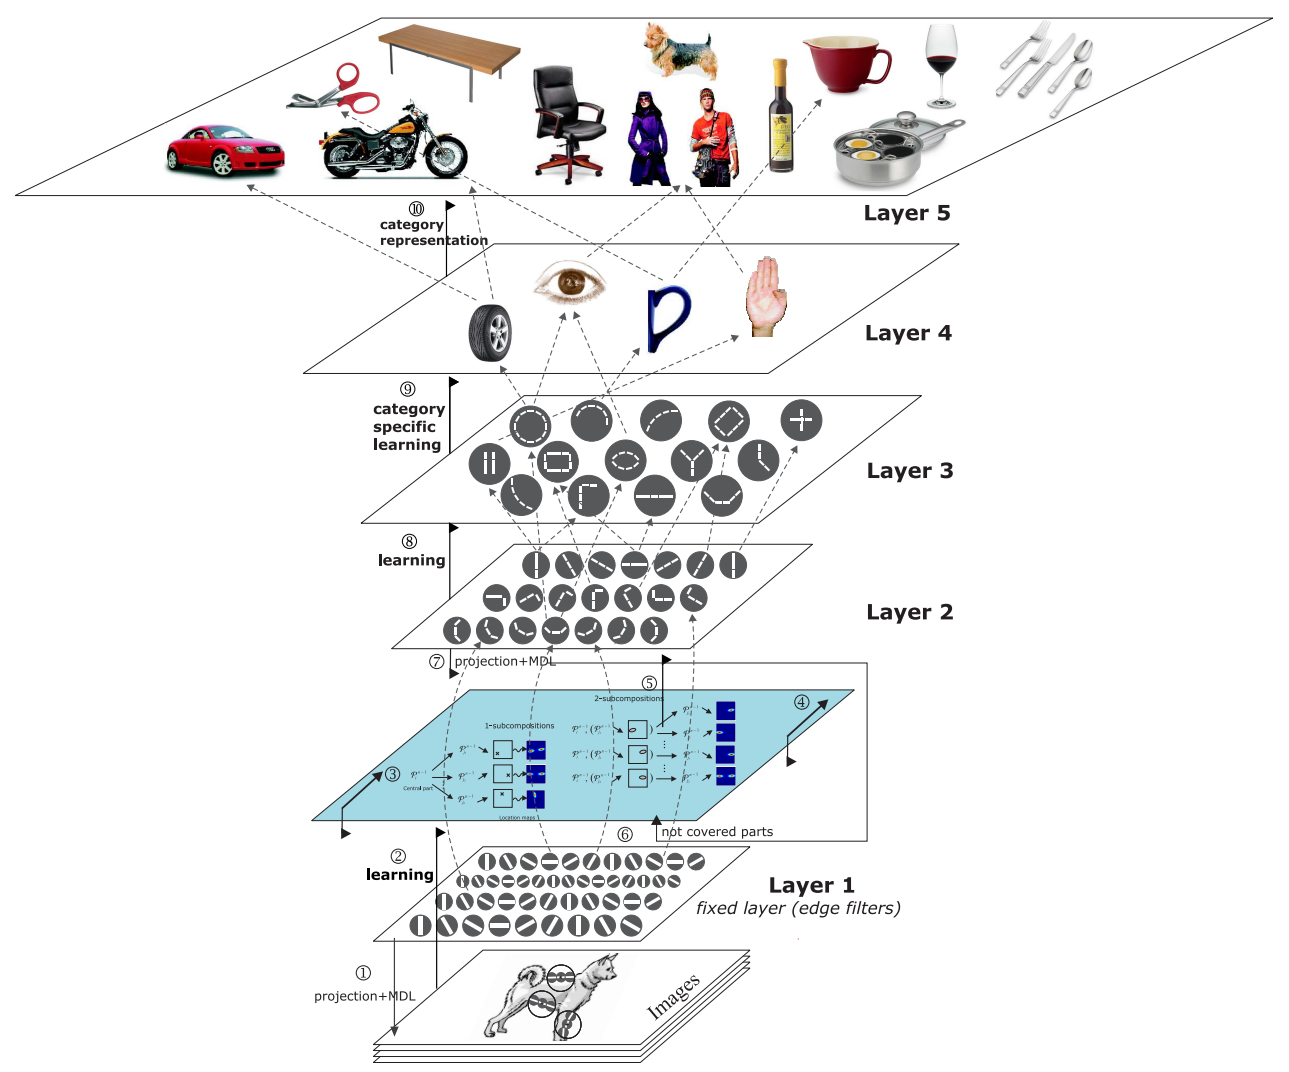
\includegraphics[width=\textwidth]{backml/image-hierarchy.png}
  \caption{A custom hierarchical model illustrating the compositionnality and hierarchical nature of vision tasks (source: \parencite{leonardis2010learning}).}
  \label{fig:backml:hierarchy}
\end{figure}

Most of the \acrlong{ml} methods developed until recently can arguably be considered
``\textit{shallow}'' which means that they are not complex enough or their learning
process does not include a mechanism to learn or exploit such hierarchies. In
order to successfully apply these methods to complex data with hierarchical
structures, one usually needs to help the learning algorithm by pre-processing
the data and extracting meaningful information using field knowledge. This process
is called \textit{manual feature extraction} or \textit{engineering} and has been
an important part of the application of machine learning algorithms. In computer
vision, a great body of work has been focused on creating complicated pipelines
of feature extraction that produce hundreds of different features that can be used
for image understanding (\eg SURF \parencite{bay2006surf}, ORB \parencite{rublee2011orb}).
However, more recently ``\acrlong{dl}'' methods based on neural networks have
shown that manual feature extraction was usually not the best performing approach
for a wide variety of tasks.

Although neural network research is as old as machine learning itself, the real
breakthrough of \acrlong{dl} happened in 2012 at the occasion of the third iteration
of a \acrlong{ml} challenge called \acrfirstit{ilsvrc} \parencite{russakovsky2015imagenet}.
One of the tasks was image classification and all but the best method used
combinations of shallow learning algorithms and feature extraction. However, the
winning team followed a different approach. Building upon neural network research
form the previous decades, they used a deep convolutional neural network, AlexNet,
trained on the raw images directly \parencite{krizhevsky2012imagenet}. They beat
the second best method by a margin of 11\% error rate. This extraordinary improvement
revived the interest of the \acrlong{ml} community for neural networks and launched
the ``\acrlong{dl} revolution''. The success of this method can be partly attributed
to some particularily beneficial \textit{inductive bias}, a set of assumptions
that narrow the search of a good model in the hypothesis space. This inductive
bias includes the use of a trainable multi-layered (hence ``deep'') structure that
can automatically learn hierarchical concepts from the data directly. In other
words, instead of manual feature engineering, features are learned automatically.
Nowadays, \acrlong{dl} is a thriving research field that has grown far beyond
image classification. Section \ref{sec:backml:deeplearning} dives a little further
into \acrlong{dl} concepts relevant to this thesis.

\subsection{Transfer learning}
\label{ssec:backml:transfer}

As humans, we have extraordinary learning capabilites. Throughout our lives, we
learn to move, communicate, interact with our environments and more. One specific
learning ability that we possess is to use knowledge we have acquired in a given
context to learn faster in a different context. For example, someone who already
plays the violin will probably feel it easier to learn to play the piano than
someone who has no music education at all. In a way, we ``transfer'' knowledge
and skills from a task to another.

This idea has been applied in \acrlong{ml} and from this application emerged
\acrfirstit{tl} \parencite{yang2020transfer}. This field studies the ways knowledge
learned from one or more tasks, called the \textit{source tasks}, can be exploited
to learn more effectively on another task, the \textit{target task}. This subject
has been researched for few decades now, as the first contributions about \acrlong{tl}
date back to the end of the 1970s \parencite{bozinovski2020reminder}. A surge of
interest happened in the 1990s notably with a NIPS-95 workshop called
``\textit{Learning to Learn: Knowledge Consolidation and Transfer in Inductive Systems}''
which discussed the importance of retaining previously-learned information for
efficient learning. Since then, the interest has only been growing and the emergence
of \acrlong{dl} has created new opportunities for \acrlong{tl}.

Transfer learning methods are organized based on the properties of the source and
target tasks. The different types of supervision (or lack thereof) discussed in
Sections \ref{ssec:backml:sl} and \ref{ssec:backml:usl} also apply to \acrlong{tl}
in which case the supervision qualifier relates to the target task only. In other
words, in supervised \acrlong{tl}, the target task is a supervised dataset as
described in Equation \ref{eqn:backml:supervised}. For the remainder of the section,
we will assume that the source tasks are also supervised.

\begin{definition}
  \label{def:backml:homotransfer}
  Transfer learning between a source task $\left(\mathcal{X}_{s}, \mathcal{Y}_{s}, p_{s}(\vect{x}, y)\right)$ and a target task $\left(\mathcal{X}_t, \mathcal{Y}_t, p_t(\vect{x}, y)\right)$ is said to be \textbf{homogeneous} when $\mathcal{X}_s \cap \mathcal{X}_t \neq \emptyset$ and $\mathcal{Y}_s = \mathcal{Y}_t$ but $p_s(\vect{x}) \neq p_t(\vect{x})$ or $p_s(y|\vect{x}) \neq p_t(y|\vect{x})$.
\end{definition}

Transfer learning can be \textit{homogeneous} (see Definition \ref{def:backml:homotransfer})
when the source and target tasks only differ by the distributions of their data.
As an example, let us suppose we would want to classify pictures taken with a
camera equipped with a certain sensor (target dataset $B$) and that we also have
at hands another dataset of pictures taken with a camera equipped with another
type of sensor (source dataset $A$). Each captor has a certain noise pattern which
results in dataset $A$ and $B$ to have a slighlty different distributions in the
pixel intensities (\ie $p_A(x) \neq p_B(x)$). This specific setup where only the
inputs distributions differ is called \textit{domain adaptation}.

\begin{definition}
  \label{def:backml:heterotransfer}
  Transfer learning between a source task $\left(\mathcal{X}_{s}, \mathcal{Y}_{s}, p_{s}(\vect{x}, y)\right)$ and a target task $\left(\mathcal{X}_t, \mathcal{Y}_t, p_t(\vect{x}, y)\right)$ is said to be \textbf{heterogeneous} when $\mathcal{X}_s \cap \mathcal{X}_t = \emptyset$ and/or $\mathcal{Y}_s \neq \mathcal{Y}_t$.
\end{definition}

Transfer learning can be \textit{heterogeneous} (see Definition
\ref{def:backml:heterotransfer}). An example that will be addressed later in this
thesis is the transfer of a model trained for natural image classification to
medical image classification. In this case, the tasks are different as the first
consists in identifying the presence of a type of object in the image whereas the
other consists in assessing the malignancy of a tumor from an image of a tissue.
The input distributions also differ as medical images have completely different
content and appearance.

There exist many different transfer approaches. Based on how they operate,
\parencite{yang2020transfer} have identified four different categories of \acrlong{tl}
algorithms. The case when knowledge transfered corresponds to the weights attached
to the source examples is called \textit{instance-based} \acrlong{tl}. Is referred
to as \textit{feature-based} \acrlong{tl} the case when knowledge is represented
by a subspace spanned by the features in the source and target domains. The
transferred knowledge can also be embedded as part of the source domain model:
this is \textit{model-based} \acrlong{tl}. Finally, when the knowledge is transferred
as rules specifying the relations between examples in the source domains, transfer
is referred to as \textit{relation-based}.

Transfer learning performance is influenced by several factors including how well
the method is able to capture and use transferable knowledge. The task-relatedness
is also an important factor: usually the more similar the tasks, the better the
performance. Sometimes, performance are worsen by the use of \acrlong{tl}. This
happens for instance when the source and target tasks are not related enough.
Moreover, the training process on the target task can cause some of the
previously-learned knowledge to be lost as most \acrlong{ml} methods do not have
an explicit memory mechanism to retain information. These two phenomena are
respectively called \textit{negative transfer} \parencite{zhang2020overcoming}
and \textit{catastrophic interference} \parencite{french1999catastrophic}. Although
some methods have been proposed to tackle these challenges, how to anticipate and
correct them are still open research questions.

We explore further \acrlong{tl} in the context of deep learning in Section
\ref{ssec:backml:dl:deeptransfer}.

\subsection{Multi-task learning}
\label{ssec:backml:mtl}

In \acrlong{tl}, the transfer process happens in two steps. First, knowledge is
extracted from the source tasks one way or another, then later used for learning
the target task. A similar approach is \acrfirstit{mtl} where, rather than performing
the transfer in two steps, everything happens at once: a model is trained on all
tasks simultaneously. Compared to learning each task individually, this approach
has several advantages: it increases the total amount of data available for training
a model, a more robust and universal representation can be learned by sharing
knowledge between tasks and, to a certain extent, it prevents the model to
overfit\footnote{See more on overfitting in Section \ref{ssec:backml:bvtradeoff}.}
a specific task. In the best scenarii, the use of \acrlong{mtl} improves the
performance of each individual task compared to a setup where the tasks are treated
independently. In opposition, it happens that antagonistic tasks worsen the
resulting individual tasks performance. This issue is related to negative transfer
and catastrophic interference introduced in Section \ref{ssec:backml:transfer}.

Similarily to \acrlong{tl}, \acrlong{mtl} methods can be either \textit{heterogeneous}
when the tasks are of different types (\eg supervised, unsupervised, classification,
regression), or \textit{homogeneous} when tasks have only one type. In supervised
\acrlong{mtl}, \cite{zhang2017survey} have identified three families of
methods. \textit{Feature-based} \acrlong{mtl} is about sharing knowledge through
learning features common among all tasks. With \textit{instance-based} \acrlong{mtl},
knowledge is shared through examples deemed useful. Finally, \textit{model} or
\textit{parameter-based} \acrlong{mtl} use learned models as proxies to extract
information about tasks relatedness.

We explore further \acrlong{mtl} in the context of deep learning in Section
\ref{ssec:backml:dl:deepmultitask}.

% ===================
% Eval and selection
% ===================

\section{Model evaluation and selection}
\label{sec:backml:modeleval}

As stated in Section \ref{sec:backml:whatisml}, evaluation is a core principle of
\acrlong{ml} as a learning algorithms should select a model that maximizes a
performance criterion. In this section, we introduce different concepts related
to the evaluation and selection of machine learning models. In Sections
\ref{ssec:backml:modelselection} and \ref{ssec:backml:bvtradeoff}, we discuss the
importance of generalization for \acrlong{ml} models and the related topics of
bias-variance trade-off and overfitting. In Section \ref{ssec:backml:modelselinpractice},
we discuss further practical consideration related to model selection. In Section
\ref{ssec:backml:metrics}, we finally introduce different metrics used in this
thesis.


\subsection{Empirical risk minimization}
\label{ssec:backml:modelselection}
As stated in the introduction, the objective of a learning algorithm is to find
a model $h \in \mathcal{H}$ that maximizes a performance measure or, alternatively,
minimizes the expected risk $R(h)$ (for a supervised problem)
\parencite{vapnik1992principles}:
\begin{equation}
\label{eqn:backml:expriskmin}
R(h) = \mathbb{E}_{\mathcal{X},\mathcal{Y}}\left\{\ell\left(y, h(\vect{x})\right)\right\}
\end{equation}
where $\ell: \mathcal{Y}\times\mathcal{Y} \rightarrow \mathbb{R}$ is a loss function
which measures the closeness between $h(\vect{x})$ and $y$. The expected risk is
also called the \textit{generalization error}. The model that minimizes $R(h)$ is
therefore the best possible model for the task and is called the Bayes model $h_B$.
In practice, it is rarely possible to directly minimize the expected risk as one
does not have access to the true distributions. It is therefore more convenient
to work with an unbiased estimator of the estimated risk, the empirical risk,
which is evaluated using the available supervised training set $\mathcal{D}$:

\begin{equation}
\label{eqn:backml:empiricalrisk}
R_e(h) = \frac{1}{n} \sum_{i=1}^{|\mathcal{D}|} \ell\left(y_i, h_\mathcal{D}(\vect{x}_i)\right), (\vect{x}_i, y_i) \in \mathcal{D}
\end{equation}

The \acrfirstit{erm} principle suggests that a learning algorithm should pick a
model that minimizes the emprical risk in order to approximate $h_B$ as well as
possible. Most machine learning algorithms apply this principle.

\subsection{Bias-variance trade-off and overfitting}
\label{ssec:backml:bvtradeoff}

Whereas it can be shown that the empirical risk, under some assumptions, converges
to the expected risk when the training set grows ($n \rightarrow \infty$), in
practice, one does not have access to an infinitely-large dataset. Therefore, the
learned model will often differ from $h_B$ and its expected risk will often be
larger. The effect of the ``\textit{choice}'' of a finite training set on the
generalization error can be studied using the \textit{bias-variance decomposition} 
\parencite{geman1992neural, geurts2009bias, hastie2017elements}:
\begin{equation}
\label{eqn:backml:biasvariancedec}
\mathbb{E}_{LS}\left\{\mathbb{E}_{\mathcal{X},\mathcal{Y}}\left\{\ell\left(y, h_{LS}(\vect{x})\right)\right\}\right\} = \text{noise}(\vect{x}) + \text{bias}^2(\vect{x}) + \text{variance}(\vect{x})
\end{equation}
where $\mathbb{E}_{LS}$ is the expectation over all training sets of size $n$ that
can be extracted from $p(\vect{x},y)$ and $h_{\mathcal{D}} \in \mathcal{H}$ is
the model learned from a learning set $\mathcal{D} \in LS$. This decomposition can
be exactly demonstrated when using the squared loss (see Equation 
\ref{eqn:backml:squaredloss}) as $\ell$. For other losses, the decomposition is not 
exactly equivalent but the intuition is similar. The \textit{noise}
term is the error of $h_B$ and is therefore irreductible. The \text{bias} is the
error of the average model (over models generated from $LS$) with respect to $h_B$.
The \textit{variance} measures the variability of the predictions around the
average model caused by the training set randomness.

Several elements have a direct impact on these error terms such as: model capacity, 
training set size, noise in the data, \etc. The \textit{capacity} or 
\textit{complexity} of a model is related to its ability to capture complex relationships 
in the data. Linear models (see Section \ref{sec:backml:svm}) are examples of low-capacity 
models as they are only able to capture linear relationships. Non-linear models such as 
random forests (see Section \ref{sec:backml:treebased}) or deep neural networks 
(see Section \ref{sec:backml:deeplearning}) have a higher complexity or capacity 
compared to linear models.

Low-capacity models usually have low variance as their limited expressiveness does
not allow them to change much based on the training data but they also have high
bias as failing to capture complex relationships prevents the model from approximating
$h_B$ correctly. This behavior is called \textit{underfitting}. In opposition,
high-capacity models have low bias as their expressiveness allow them to approximate
$h_B$ more accurately but this expressiveness also leads to high variance as the
model can learn a function which is too expressive compared to $h_B$ and can fit
the noise in the training data. Such models suffer from \textit{overfitting} which
hampers generalization, although these models typically present a low empirical
risk. The \textit{bias-variance trade-off} results from these observations and
states that finding a model that generalizes consists in finding the trade-off
between low- and high-capacity or underfitting and overfitting. In Figure
\ref{fig:backml:biasvariancetradeoff} is plotted the classical representation of
this trade-off.

\begin{figure}
  \centering
  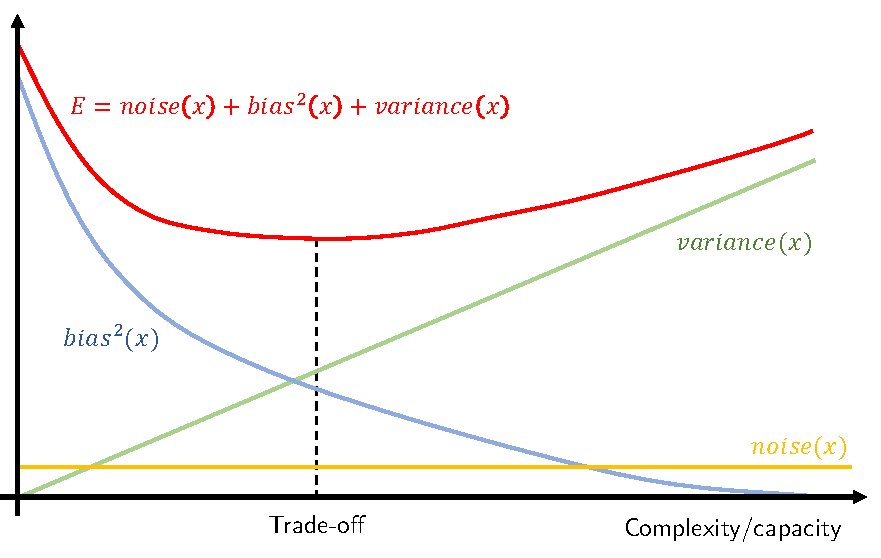
\includegraphics[width=0.75\textwidth]{backml/biasvariancetradeoff.pdf}
  \caption{The bias-variance trade-off illustrated.}
  \label{fig:backml:biasvariancetradeoff}
\end{figure}

\subsubsection{Over-parametrized models}

With the advent of \acrlong{dl}, model complexity has exploded as typical \acrlong{dl}
models have millions or even billons of parameters (see Section
\ref{ssec:backml:dl:modernarchi}). The bias-variance trade-off tells us that these
models should be extremely prone to overfitting but the reality is different.
Typically, it is not uncommon to find tasks for which \acrlong{dl} models reach
an empirical risk close to zero but actually generalize well to unseen data
\parencite{zhang2021understanding}. Although the models are able to basically
memorize the training data, the learned function is actually very robust and
generalize well. This phenomenon is currently being investigated and several
explanations have been proposed such as the deep double-descent
\parencite{belkin2019reconciling}.

\subsection{Model selection and evaluation in practice}
\label{ssec:backml:modelselinpractice}

These considerations have direct consequences on practical applications of machine
learning. In particular, the presence of overfitting causes the empirical risk to
reflect poorly the generalization error of a model. There are two common tasks
where using the empirical risk only is not reliable which are \textit{model selection}
and \textit{model evaluation}. The former consists in finding the model that would
generalize best among a set of candidates and the latter consists in evaluating
the expected performance of a model when it will be used on new data. Both tasks
involve evaluating the generalization error of a model. There exist several approaches
to solve these tasks.

The simplest one is the use of an independent test set: the source dataset is
split into two subsets, the train and test sets, which are used to respectively
train and evaluate the model. The size of the subsets should be made such that
the train set is large enough for the model to be able to learn but the test set
should be large enough for the estimate of the error to be reliable. Those two
objectives are obviously antagonistic. Therefore, this approach is not viable if
the source dataset is too small as reducing even more the size of the sets will
make both the training and evaluation unreliable. The test-set approach actually
evaluates the generalization error of the model for the given dataset but not the
expected generalization error presented in Equation \ref{eqn:backml:biasvariancedec}.

Another approach that actually estimates the expected generalization error is
\acrfirstit{cv} which simply repeats the train-test approach with different splits
of the source dataset. For each train-test split, a model is trained on the train
set and evaluated on the test set. The \acrlong{cv} score is computed by averaging
the test scores of all splits. There exist several approaches for \acrlong{cv}
which differ by how they generate their splits. A common approach is
\textit{$k$-fold \acrlong{cv}} where the data is randomly split into $k$ subsets
and each subset is selected in turn to be the test set while the remaining folds
make the train set.

An important consideration is to never use a model selection score as the evaluation
score of a model. Indeed, optimizing the choice of a model usually results in the
selection score to be an overly optimistic estimator of the generalization
performance of the model. In practice, this results in a three-way split of the
training dataset: one extracts some train, validation and test sets. The models
are trained on the train set, selected on the validation set and the final model
is evaluated on the test set. When the dataset is too small for such a three-way
split, a common approach consists in extracting a test set from the whole dataset
and then performing \acrlong{cv} on the train set. As a general rule, every decision
influenced one way or another by the output $y$ should be done within a validation
loop to avoid overfitting (using either \acrlong{cv} or an independent
test-set).

These two approaches are based on a strong assumption that the extracted sets are
independent. If they are not, this would most probably lead to overfitting and
the resulting selection or evaluation scores being overly optimistic. Therefore,
it is sometimes not enough to split the sets randomly and domain knowledge must
be used during the splitting procedure to enforce sets independance. This issue
is sometimes called \textit{data leakage} \parencite{kaufman2012leakage} as
information ``leaks'' between the sets. This topic will be discussed in Section
\ref{ssec:backdp:dataleakage} as \acrlong{dp} datasets must treated carefully to avoid
this issue.

\subsection{Metrics}
\label{ssec:backml:metrics}

% F1 ?
The metrics presented in this section are mostly supervised classification
performance measures. Given a supervised dataset as described in Equation
\ref{eqn:backml:supervised}, the metrics evaluate how the predicted class $\hat{y}_i$
compares to the ground truth class $y_i$. In the remainder of the thesis, when
the higher the better for a metric, we will call it a \textit{score}. In opposition,
when the lower the better, we will call it a \textit{loss}. In terms of notations,
a loss and a score averaged over a set of data will respectively be noted
$\mathcal{L}$ and $\mathcal{M}$.

\subsubsection{Accuracy}
\label{sssec:backml:metric:acc}
The accuracy was introduced in our first example of a machine learning problem in
Section \ref{sec:backml:whatisml} with its dual, the zero-one loss. The accuracy
assigns 1 to correct predictions and 0 to misclassified samples. The accuracy
score can be computed over a dataset:

\begin{equation}
\label{eqn:backml:accuracy}
\mathcal{M}_{\text{acc}} = \dfrac{1}{n} \sum\limits_{i = 1}^n (1 - \ell_{\text{0-1}}(y_i, \hat{y}_i))
\end{equation}

It has the advantage of being simple to interpret, to compute and it applies to
both binary and multi-class problems. However, it is affected by \textit{class imbalance}.
This phenomenon designates the situation when there is a disparity in the numbers
of examples belonging to each of the problem classes in the dataset. For instance,
given binary dataset where $n-1$ examples belong to class $A$ and the last example
to class $B$, a classifier predicting only class $A$ would obtain an accuracy
close to $1$ which seems very good but in reality the classifier did not learn
anything from the data.

\subsubsection{Area under the ROC curve}
\label{sssec:backml:metric:rocauc}

In binary classification, a specific name is given to each type of successful or
unsuccessful predictions and these different types of successes and errors form
what is called the \textit{confusion matrix} (see Table \ref{tab:backml:confusion}).
Each element of this table can be either a number or a proportion of samples
falling in the category. The accuracy presented in Section \ref{sssec:backml:metric:acc}
can be re-expressed based on this confusion matrix: $\frac{TN + TP}{N + P}$. In
some context, however, it is more informative to look at other types of errors.
For instance, when the target task consists in diagnosing cancer, one is more
interested in assessing the number of false positives and negatives of the method
using, for instance, the \textit{specificity} or \textit{sensitivity} (\aka recall)
scores.

\begin{equation}
\label{eqn:backml:specifity}
\textit{Specifity} = \frac{TN}{TN + FP} = 1 - \frac{FP}{N}
\end{equation}

\begin{equation}
\label{eqn:backml:sensitivity}
\textit{Sensitivity} = \frac{TP}{P}
\end{equation}

\begin{table}
  \centering
  \begin{tabular}{c|cc|c}
  & \multicolumn{2}{c}{Predicted ($\hat{y}$)} & \\
  Actual ($y$) & 0 & 1 & Total \\
  \hline
  0 & \textbf{T}rue \textbf{N}egative & \textbf{F}alse \textbf{N}egative & \textbf{N}egative \\
  1 & \textbf{F}alse \textbf{P}ositive & \textbf{T}rue \textbf{P}ositive & \textbf{P}ositive \\
  \end{tabular}
  \caption{A confusion matrix for a binary classification problem.}
  \label{tab:backml:confusion}
\end{table}

\textit{Sensitivity} and $1 - \textit{specificity}$ are also called \acrfirstit{tpr}
and \acrfirstit{fpr} respectively. These metrics should always be studied together
as it is often possible to optimize one at the expense of the other. Therefore a
common analysis consists in plotting a model as a point $(\acrshort{tpr}, \acrshort{fpr})$
in a two-dimensional graph. Some classification models are able to produce class
probabilities instead of just a class. In this case, one can vary a threshold
applied to these probabilities in order to generate several points to plot. These
points form a visual metric called the \acrfirstit{roc} curve (see Figure
\ref{fig:backml:roc-curve}) which can be derived into a score: the
\textit{area under the \acrshort{roc} curve} (\rocauc). This
score can only be computed for model which produce a meaningfully
thresholdable number and it only applies to binary classification in its basic form.
However, it provides a measure which is not impacted by class imbalance which is
a very interesting property in domains where this issue is common. Another advantage
of the \rocaucs is its finer grasp of how a model performs as it evaluates
the probabilities unlike the accuracy where the model is either wrong or right but
there is no in-between.

\begin{figure}
  \centering
  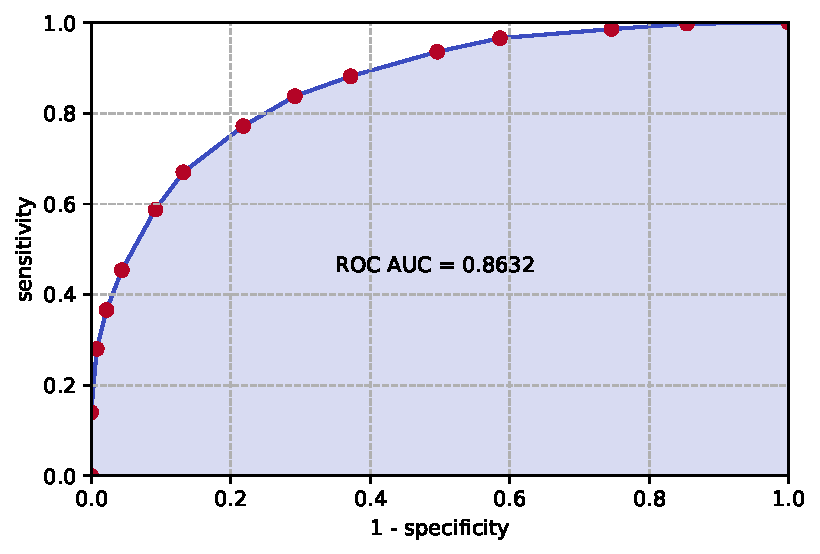
\includegraphics[width=0.65\textwidth]{backml/roc-curve.pdf}
  \caption{A \acrshort{roc} curve. The red points correspond to different threshold values applied to the probabilities produced by the model. The area of the light blue zone under the curve is the \acrshort{roc} \acrshort{auc} score.}
  \label{fig:backml:roc-curve}
\end{figure}


\subsubsection{Cross-entropy loss}
\label{sssec:backml:metric:crossentropy}

Cross-entropy is rooted in information theory and measures the similarity of two
probability distributions $p$ and $q$ that, when defined over a finite and discrete
set of events $\mathcal{X}$, is given by:
\begin{equation}
\label{eqn:backml:crossentropy}
H(p, q) = - \sum\limits_{x_i \in \mathcal{X}} p\left(x_i\right) \log q\left(x_i\right)
\end{equation}

When the model outputs class probabilities, this similarity measure can be used
to evaluate the discrepancy between the prediction and the ground-truth. The
cross-entropy becomes a loss function called the
\textit{categorical cross-entropy}:
\begin{equation}
\label{eqn:backml:crossentropyloss}
\mathcal{L}_{ce} = - \frac{1}{n} \sum\limits_{i=1}^n \sum\limits_{c=1}^{\left|\mathcal{Y}\right|} y^{(c)}_{i} \log \hat{y}^{(c)}_i
\end{equation}
where $\hat{y}^{(c)}_i$ is the probability predicted by the model for example $i$
and class $c$ and $y^{(c)}_i$ is the one-hot encoding of the ground truth:
\begin{equation}
\label{eqn:backml:onehotencoding}
y^{(c)}_i =
\begin{cases}
1,\,\text{if}\, y_i = c \\
0,\,\text{otherwise}
\end{cases}
\end{equation}

In the case of binary classification, the metric falls back to the
\acrfirstit{bce}:
\begin{equation}
\label{eqn:backml:bce}
\mathcal{L}_{bce} = - \frac{1}{n} \sum\limits_{i=1}^n \left(y_i \log \hat{y}_i + (1 - y_i) \log (1 - \hat{y}_i)\right)
\end{equation}

Similarly to \rocauc, the cross-entropy evaluates probabilities and therefore has
a fine grasp on how the model performs. Another important advantage is its
differentiability as it can be used as a loss for directly training differentiable
models (\eg \acrlong{dl} models, see Section \ref{ssec:backml:dl:opti}).

\subsubsection{Dice score}
\label{sssec:backml:metric:dice}

As opposed to the previous metrics, the dice score is a set similarity measure
that is used to evaluate binary image segmentation. Considering two sets $\mathcal{A}$
and $\mathcal{B}$, the dice score is defined as:
\begin{equation}
\label{eqn:backml:diceAB}
Dice = \frac{2 \left|\mathcal{A}\cap \mathcal{B}\right|}{\left|\mathcal{A}\right| + \left|\mathcal{B}\right|}
\end{equation}
When working with image segmentation, $\mathcal{A}$ and $\mathcal{B}$ become the
sets of true and predicted binary labels for the pixels in the image and the
intersection falls back to a dot product. The resulting formula is:
\begin{equation}
\label{eqn:backml:dice}
\mathcal{M}_{dice} = \dfrac{2 \sum_i\sum_j y_{ij} \hat{y}_{ij} + \epsilon}{\sum_i\sum_j y_{ij} + \sum_i\sum_j \hat{y}_{ij} + \epsilon}
\end{equation}
where $\epsilon$ is a small value added for numerical stability, $y_{ij}$ is the
actual class of pixel $(i, j)$ and $\hat{y}_{ij}$ the predicted class for this
pixel. The predicted $\hat{y}_{ij}$ can either be binary or a probability. In the
latter case, the metric is called the \textit{soft dice score} which is differentiable.
When the model outputs class probabilities, instead of using the soft dice score,
$\hat{y}_{ij}$ can be binarized using a threshold.

\subsubsection{Rankings of metrics}
\label{ssec:backml:metric:rankings}

In Part \ref{part:transfer} of this thesis, we use a relatively large set of image
classification datasets to study \acrlong{tl}. In order to compare the different
methods, we evaluate how it performs on those datasets. Unfortunately, for reasons
that will be explained later, it is not possible to use the same metric for all
datasets. Moreover, a metric computed on a dataset is not always comparable to
the same metric computed on a different dataset. For this reason, we resort to
using \textit{rankings of methods}. First, for each dataset in our pool, we evaluate
the methods each with their most appropriate metric and then rank them: the best
method gets rank 1 and the worst gets rank $m$ (where $m$ is the number of methods).
Finally, in order to draw general conclusions, we average the rankings over all
the datasets. The average ranks therefore provides a single metric for comparing
the methods across datasets.

% ===================
% Methods
% ===================

\section{Support vector machines}
\label{sec:backml:svm}

The \acrfirstit{svm} binary classification algorithm was invented in the early 1990s \parencite{boser1992training}.
It is originally a linear binary classification method that has been extended for regression and multi-class classification.
By using the \textit{kernel trick}, \acrshort{svm} can also learn non-linear models
but it is out of the scope of this thesis. An interested reader will learn more
about kernel methods and the kernel trick in \parencite{hastie2017elements}.

In general, assuming a supervised dataset where inputs are such that
$\vect{x} \in \mathbb{R}^m$ where $m$ is the number of features, a linear model
is an hyperplane:

\begin{equation}
\label{eqn:backml:linearmodel}
f(\vect{x}) = \theta_0 + \sum_{j=1}^m \theta_j x_j
\end{equation}

where $\theta_0$ and the $\theta_j$ are the learnable parameters, respectively
called the \textit{bias} and the \textit{weights}. This model can be used for
regression in which case the model $h(\vect{x}) = f(\vect{x})$. A linear model
can also be used for binary classification in which case the linear function is
called the \textit{decision boundary} and is considered to separate positive from
negative samples in the input space: $h(\vect{x}) = \text{sign}(f(\vect{x}))$ (\ie
$\mathcal{Y} = \left\{-1, 1\right\}$). Linear methods differ from each other by
the way they learn and generate these weights.

Support vector machines optimize the parameters $\theta_0$ and $\theta_j$ to
generate $f$ in such a way that the minimal distance from the hyperplane to the
nearest points from the learning set is maximized. These nearest points are called
the \textit{support vectors} and the margin between the support vectors is called
the \textit{gutter}. An example of a \acrshort{svm} hyperplane is given in Figure
\ref{fig:backml:svm}. It can be shown that the \acrshort{svm} optimization problem
falls back to the Lagrange dual:

\begin{align}
\label{eqn:backml:svmoptimizationproblem}
\underset{\boldsymbol{\alpha}}{\text{max}}& \sum_{k=1}^n \alpha_k - \frac{1}{2} \sum_{i,j=1}^n \alpha_i\alpha_j y_i y_j \vect{x}_i^T \vect{x}_j \\
\text{subject to}~& 0 \leq \alpha_k \leq C, \forall k = 1, ..., n \\
& \sum_{i=1}^n \alpha_i y_i = 0
\end{align}
which can be solved efficiently with classical linear solvers such as LIBLINEAR
\parencite{fan2008liblinear}. When the optimal solution has been found, the weights
can be derived by solving the system:
\begin{equation}
\label{eqn:backml:svmweights}
\alpha_k\left(y_k \left(\theta^T \vect{x}_k + b\right) - 1\right) = 0, \forall k = 1, ..., n
\end{equation}
and the final model written as:
\begin{equation}
  h(\mathbf{x}) = \sum_{i=1}^m \alpha_i y_i \mathbf{x}_i^T\mathbf{x} + b
  \label{eqn:backml:finalsvmmodel}
\end{equation}

In Equation \ref{eqn:backml:svmweights}, $\alpha_k > 0$ for the support vectors
$x_k$ and $\alpha_k = 0$ for the other samples. This is an interesting property
as it implies that only the support vectors and their weights $\alpha_k$ should
be stored for future inference. This makes the final model (see Equation \ref{eqn:backml:finalsvmmodel}) 
very memory efficient for
problems where $m \gg n$. This property has also a negative side effect as it
means that the model is highly dependent on the support vectors $x_k$. It can
therefore change significantly if the $x_k$ are removed or changed which yields
high variance.

The $C$ term in the Lagrange dual formulation is an hyperparameter that relaxes
the need for linear separability of the training data and allows for training
examples to lie within the gutter or to be misclassified. Low values of $C$ make
the optimal solution tolerate more of such examples. Reducing the dependency of
the model on very few points also decreases the variance but increases the bias.
In opposition, high values of $C$ puts a large penalty on points that lie withing
the gutter or are misclassified which increases variance but decreases bias.

\begin{figure}
  \centering
  \begin{subfigure}[t]{0.48\textwidth}
    \centering
    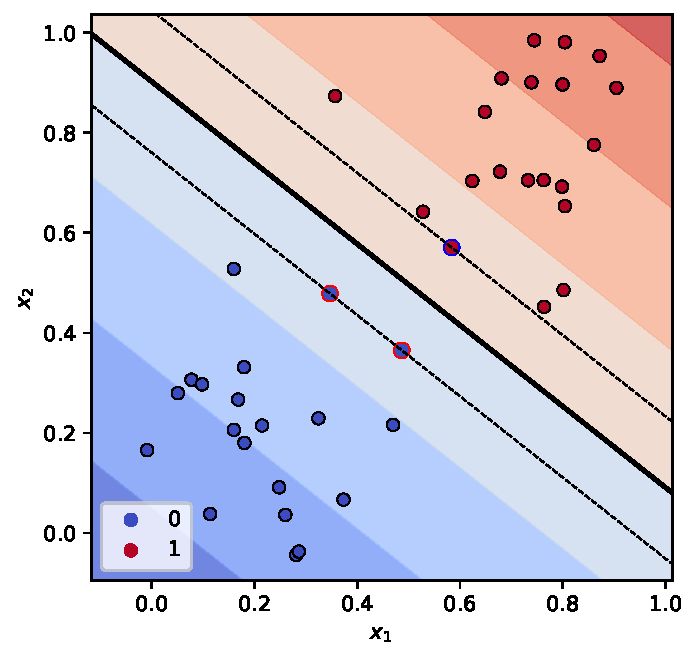
\includegraphics[width=\textwidth]{backml/svm_c10000.pdf}
    \caption{$C=10000$}
  \end{subfigure}
  \begin{subfigure}[t]{0.48\textwidth}
    \centering
    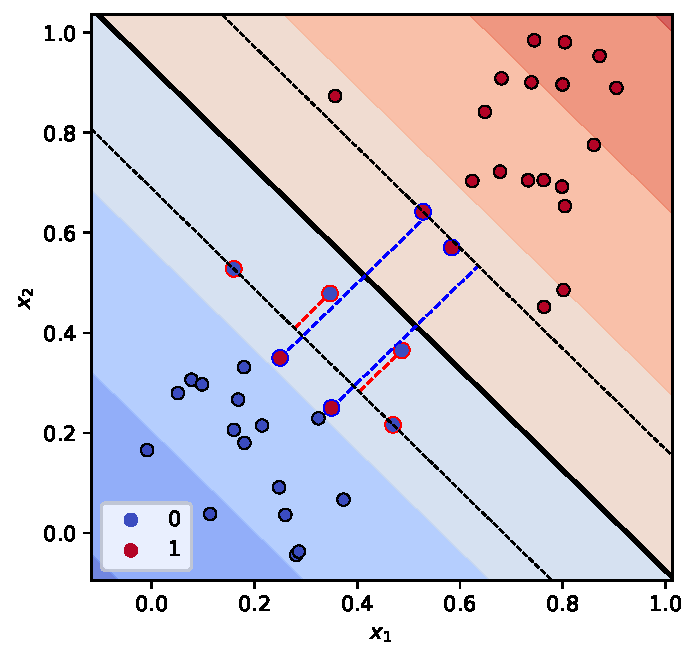
\includegraphics[width=\textwidth]{backml/svm_c25.pdf}
    \caption{$C=25$. Notice the new points \\ of class $1$ in the class $0$ cluster.}
  \end{subfigure}
  \caption{Examples of an hyperplane (the thick black line) learned with \acrshort{svm} applied to a binary classification task ($\vect{x} = (x_1, x_2) \in \mathcal{X} \subseteq \mathbb{R}^2$ and $\mathcal{Y} = \left\{0, 1\right\}$). The support vectors are delineated with bold coloured border. A large value of $C$ penalizes more severely points in the gutter or misclassified.}
  \label{fig:backml:svm}
\end{figure}


\subsection{Multi-class problems}

There exist few approaches to use a binary classification algorithm like
\acrshort{svm} in a multi-class context. One of them is called \acrfirstit{ovo}
and consists in training $K=\frac{C(C-1)}{2}$ binary classifiers (where $C$ is
the number of classes), one for each pair of classes of the dataset. The prediction
for a new sample will be the majority class among the predictions of these $K$
models. This requires learning a model number quadratic with regard to the number
of classes. When C is large, this can be quite inefficient.

Another approach is called \acrfirstit{ovr} and consists in training $C$ models
each of which deals with the classification problem of a class versus all the
others. The final prediction is given by the model of which the decision function
returned largest value. This approach is more computationally efficient than
\acrshort{ovo} as only $C$ classifier have to be trained.

\section{Tree-based methods}
\label{sec:backml:treebased}

Tree-based methods are a popular family of methods invented at least twice in the
1980s by the \acrshort{ai} \parencite{quinlan1986induction} and the statistics
\parencite{breiman1984classification} communities. Section \ref{ssec:backml:dt}
presents the basics of decision tree inference and induction, Section \ref{ssec:backml:rf}
introduces the random forest algorithm. Section \ref{ssec:backml:et} presents a
variant of random forest called \acrfirstit{et} and Section \ref{ssec:backml:et_image}
finally explores how this method can be used for image classification.

\subsection{Decision trees}
\label{ssec:backml:dt}

Let us consider a supervised dataset where each $\vect{x}_i$ is a vector of
attributes:
\begin{equation}
\label{eqn:backml:dt:vectattributes}
\vect{x}_i = \left(a^{(i)}_1, a^{(i)}_2, ..., a^{(i)}_m\right),~a^{(i)}_j \in \mathcal{X}_j
\end{equation}
and each attribute can be either numerical or categorical (binary or multi-valued).
A decision tree is a model structured as a tree of which the nodes $\mathcal{Q}$
are divided in two subsets: the internal and leaf nodes $\mathcal{I} \subset \mathcal{Q}$
and $\mathcal{F} \subset \mathcal{Q}$. Each internal node $q \in \mathcal{I}$
tests an input attribute $q.k \in \left\{1,...,m\right\}$ and its $q.E$ outwards
edges are associated with non-overlapping subsets of this attribute's domain:
\begin{equation}
\label{eqn:backml:dt:splitsgeneric}
\mathcal{A}^{(q)}_l \subset \mathcal{X}_{q.k},~l = 0,...,q.E-1
\end{equation}
which are called \textit{splits}. A leaf node of the tree is labelled with a
prediction $\hat{y} \in \mathcal{Y}$. In classification, it can also be a probability
distribution over $\mathcal{Y}$. In regression, the output is a real value
$\hat{y} \in \mathcal{Y}$. Given $x_i$, predicting an output value consists in a
top-down traversal of the tree. When reaching an internal node $q$ during the
traversal, $\vect{x}_i$ will follow the edge $l$ such that $a^{(i)}_{q.k} \in \mathcal{A}^{(q)}_l$
which leads to one of the children nodes of $q$. This process is repeated until
the algorithm reaches a leaf of which the associated labelling is the output of
the algorithm for $\vect{x}_i$.

In the remainder of the thesis, we will only consider numerical attributes ($x_i \in \mathbb{R^m}$) and
binary splits at each internal node ($q.E = 2$). These splits are defined by a
threshold $q.v$ such that:
\begin{align}
\label{eqn:backml:dt:splitsbinary}
\mathcal{A}^{(q)}_0 &= \left]-\infty, q.v\right]\\
\mathcal{A}^{(q)}_1 &= \left]q.v, +\infty\right[
\end{align}
This representation allows for an efficient check at each node as the attribute
has just to be compared to the treshold. The inference algorithm is formalized in
Algorithm \ref{algo:backml:dtinference} for classification with numerical
attributes.

\begin{algorithm}[t]
  \SetAlgoLined
  \KwData{A sample $\vect{x}_i = \left(a^{(i)}_1, a^{(i)}_2, ..., a^{(i)}_m\right)$ and the root $r$ of a decision tree.}
  \KwResult{A probability distribution over $\mathcal{Y}$, the prediction for $\vect{x}_i$.}
  \SetKwFunction{dtinfer}{TreeInference}
  \Fn{\dtinfer{$r$, $\vect{x}_i$}}{
    $q = r$\;
    \While{$q \not\in \mathcal{F}$}{
      \eIf{$a^{(i)}_{q.k} \leq q.v$}{
        $q = q.\text{left}$\;
      }{
        $q = q.\text{right}$\;
      }
    }
    \KwRet{$q.\text{pred}$}\;
  }
  \caption{Inference with a classification tree and numerical attributes. $q.\text{left}$ and $q.\text{right}$ denote the left and right children of a node $q$ and the prediction associated with the leaf node $f \in \mathcal{F}$ is accessed through $f.\text{pred}$. The regression algorithm only differs by its type of output.}
  \label{algo:backml:dtinference}
\end{algorithm}

\subsubsection{Decision tree induction}
\label{sssec:backml:dtinduction}

Top-down tree induction is the name of the process of building a decision tree
from a supervised dataset. It is a greedy algorithm that, for a node and a set of
examples $S$, will select an attribute and a split which reduce the most the
so-called \textit{impurity} of the node. Then, $S$ will be divided in two subsets
$S_0$ and $S_1$ based on the selected split and these will be used to build
recursively the left and right sub-trees respectively. This procedure is repeated
until a certain stopping criterion is met. An impurity measure $I(S)$ evaluates
the disparity of the output labels $y_i$ in a set $S$ of training examples. For
classification, a common impurity measure is the Shannon entropy computed on the
class frequencies $p_i$:
\begin{equation}
\label{eqn:backml:shannon_entropy}
I(S) = - \sum_{i=1}^C p_i \log p_i
\end{equation}
The simplest stopping criterion would be to stop developing the tree when the
subset at the node cannot be further divided because either it is pure (\eg only
one class represented in $S$) or because all attributes have a constant value.
This algorithm is formalized in Algorithm \ref{algo:backml:dtinduction}.


\begin{algorithm}[t]
  \SetAlgoLined
  \SetKwFunction{dtinduct}{TreeInduction}
  \SetKwFunction{stopsplit}{StopSplit}
  \SetKwFunction{computepred}{ComputePred}
  \KwData{A  supervised dataset $S$ where each sample $\vect{x}_i = \left(a^{(i)}_1, a^{(i)}_2, ..., a^{(i)}_m\right)$.}
  \KwResult{The root node of a decision tree built for $S$.}

  \Fn{\dtinduct{$S$}}{
    \If{\stopsplit($S$)}{
      \KwRet{\text{a node associated with the most appropriate labelling given} $S$}\;
    }
    Find the best split $q.v$ for attribute $q.k$ for new node $q$:\;
    $\argmin{v,k} \left[\frac{|S_0|}{|S|} I\left(S_0\right) + \frac{|S_1|}{|S|} I\left(S_1\right)\right] : S_0 = \left\{(\vect{x}_i, y_i) \mid a^{(i)}_k < v\right\}, S_1 = S \setminus S_0 $\; \label{algo:backml:dtinduction:argmax}
    $q.\text{left} =~$\dtinduct{$S_0$}\;
    $q.\text{right} =~$\dtinduct{$S_1$}\;
    \KwRet{$q$}\;
  }
  \;
  \Fn{\stopsplit{$S$}}{
    \KwRet{$true~$\text{if either the $y_i$ or all the attributes are constant in} $S$, $false~$\text{otherwise}}\;
  }
\caption{Decision tree induction.}
\label{algo:backml:dtinduction}
\end{algorithm}

\begin{figure}
  \centering
  \begin{subfigure}[t]{0.48\textwidth}
    \centering
    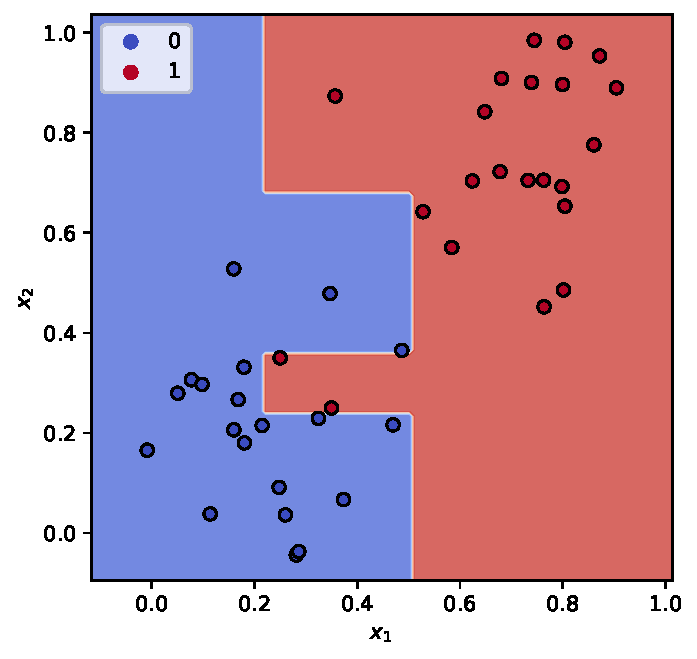
\includegraphics[width=\textwidth]{backml/dt_full.pdf}
    \caption{Fully-developped}
  \end{subfigure}
  \begin{subfigure}[t]{0.48\textwidth}
    \centering
    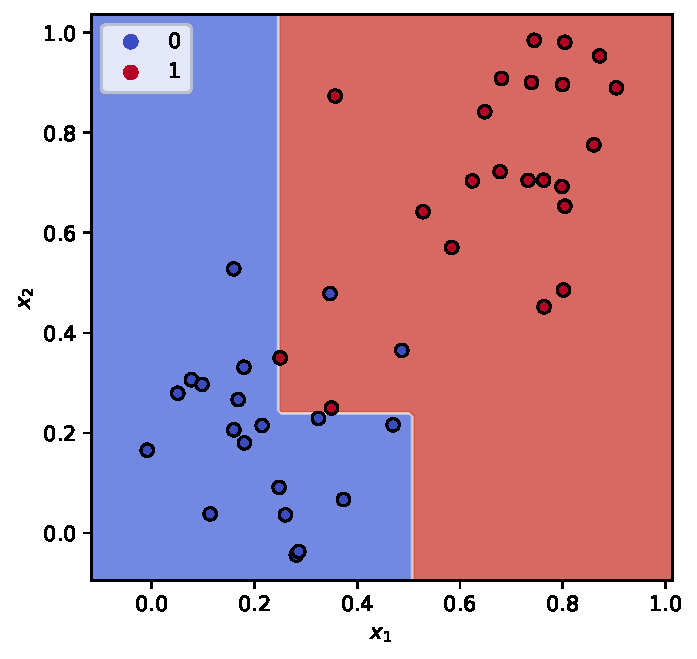
\includegraphics[width=\textwidth]{backml/dt_max_depth3.pdf}
    \caption{Maximum depth = 3}
  \end{subfigure}
  \caption{Decision tree decision boundary (white line). Pre-pruning using the maximum depth parameter reduces the complexity of the model.}
  \label{fig:backml:dt_boundary}
\end{figure}

A tree built using this simple stopping criterion is said to be \textit{fully-developed}.
Such a tree is able to capture the training set perfectly which, in practice,
hurts generalization as it usually leads to overfitting. In order to alleviate
the problem and reduce the variance, there exist several methods such as pre-pruning
which consists in preventing the final tree to grow too deep. Simple pre-pruning
techniques are, for example, stopping the induction when a branch reaches a certain
depth, or ensuring that all leaf nodes contain at least a given number of samples
(see Figure \ref{fig:backml:dt_boundary}). An advantage of decision trees are
their interpretability as the rules learned by the model can be easily understood
by looking at the tree. In practice, decision trees are rarely used alone because
of their high variance.

\subsection{Random forests}
\label{ssec:backml:rf}

Random forests \parencite{breiman2001random} is an ensemble method based on decision
trees. Ensemble methods combine the predictions of several models to produce a
final prediction. Random forest is part of the family of averaging techniques
where models are built independently and their predictions are averaged (\eg a
majority vote for classification). It can be shown that this approach reduces
variance compared to that of the base model (\eg decision trees) and the more
decorrelated the individual models, the larger the variance reduction.

In random forests, decorrelation is achieved through \textit{bagging} (\aka
bootstrap aggregating) and \textit{random attribute subset selection}. The former
consists in training each individual model on a bootstrap sample of the training
set: the training set for the $t^{\text{th}}$ decision tree in the ensemble is a
set $S_t$ built by sampling $n$ examples with replacement from the original training
set $S$. Regarding the attribute subset selection, each tree only considers a
subset of $K \in \left\{1,..., m\right\}$ randomly selected features when looking
for the best split. In other words, only $K$ random features are considered when
searching for $q.k$ at line \ref{algo:backml:dtinduction:argmax} in Algorithm
\ref{algo:backml:dtinduction}. These two sources of randomness usually increase
the bias as the individual models do not have access to all the original training
examples and attributes. However, the variance reduction resulting from ensembling
is usually of much greater magnitude resulting in a significant performance
improvement compared to using a decision tree alone.

\subsection{Extremely randomized trees}
\label{ssec:backml:et}

The \textit{\acrlong{et}} (\acrshort{et}, \aka extra-trees) \parencite{geurts2006extremely}
are a variant of the random forests algorithm that introduces yet another source
of decorrelation by selecting the split $q.v$ at random during the induction
(instead of optimizing it, see line \ref{algo:backml:dtinduction:argmax} in
Algorithm \ref{algo:backml:dtinduction}). Moreover, to attenuate the bias increase,
each individual tree is built on the whole training set instead of a boostrap
sample. These choices makes the algorithm particularily computationally efficient
as it is not necessary to iterate over the training samples to optimize the split
anymore.

\subsection{Image classification with extra-trees}
\label{ssec:backml:et_image}

Extra-trees can be used for image classification as presented in \parencite{maree2016towards}.
The core idea behind this algorithm is to represent an image as a set of $n_w$
random subwindows. Subwindows are rectangle patches extracted from the image,
resized to have all the target height $t_r$ and width $t_c$ and flattened into a
vector of dimension $t_r \times t_c \times b$ ($b$, the number of color channels,
or bands, in the image). The original dimensions of the rectangular patches are
drawn uniformly at random in a range of proportions $s_{min}$ and $s_{max}$ of
the image size ($0 \leq s_{min} < s_{max} \leq 1$). The position of the patches are
also drawn uniformly at random. Each subwindow is attributed the class of its
parent image. The resulting training dataset containing $n \times n_w$ examples,
each a vector of dimension $t_h \times t_w \times c$, can be used to train an
extra-trees classifier. At inference, the same extraction process is applied and
the final prediction for the image is determined by a majority vote on the predicted
classes for its subwindows. Regarding parameters, the more windows and the more
trees in the forest, the better. In addition to the tree complexity hyperparameters,
the image colorspace, $s_{min}$ and $s_{max}$ should be tuned as well to optimize
generalization.

This variant of the algorithm is called \acrfirstit{etdic} but another variant
exists where the forest is used as a feature-learner (\acrshort{etfl}). The idea
of \acrshort{etfl} is to train a limited number of trees with the subwindows
dataset similarly to the \acrshort{etdic} approach. But rather than using the
forest as a direct classifier, it is used to create a new representation for the
images. This representation is a vector of the same dimension as the number of
leaves in the forest and value $\nu_i$ for leaf $i$ corresponds to the frequency
of subwindows of the image reaching the leaf when propagated into the forest. This
representation can then be used to train another classifier like \acrshort{svm}.
At inference, the representation for the new samples is extracted from the forest
which are then classified with the second classifier. In general, \acrshort{etfl}
is superior to \acrshort{etdic} in terms of performance.

\section{Deep learning}
\label{sec:backml:deeplearning}

As introduced in Section \ref{ssec:backml:shallowdeep}, \acrlong{dl} is a broad
research field that has grown rapidly since the breakthrough of AlexNet in 2012.
It encompasses many different research topics covering all areas of machine
learning. In this section, we dive further in \acrlong{dl} concepts and
methods relevant to this thesis. We introduce the basic components of modern neural
network architectures in Section \ref{ssec:backml:dp:components}. Section
\ref{ssec:backml:dl:opti} discusses how neural networks are learned and optimized
in practice. Section \ref{ssec:backml:dl:modernarchi} presents few modern neural
network architectures. Finally, in Section \ref{ssec:backml:dl:deeptransfer}, we
discuss deep \acrlong{tl}.

\subsection{Components of modern neural networks}
\label{ssec:backml:dp:components}

A feedforward neural network can be seen as a parametrized function approximator
$h$ which combines several intermediate functions $h^{(l)}(\cdot, \theta^{(l)})$
($l=1, ..., L$), also called \textit{layers}, through composition:
$h(\vect{x}, \theta) = (h^{(L)} \circ h^{(L-1)} \circ ... \circ h^{(1)})(\vect{x})$.
$\theta$ is the set containing all the learnable parameters of the neural network
$h$ and $\theta^{(l)}$ are the parameters of the function $h^{(l)}$ (or layer
$l$). The feedforward nature of the network specifies that information only flows
one-way, from the input $\vect{x}$ to the output $y$. In other words, there is no
feedback loop.

Unlike decision trees, for instance, which learn the tree structure automatically,
the architecture of a neural network is built manually (most of the time) and
consists in choosing and combining the appropriate functions $h^{(l)}$ for the
task at hand. Although it introduces some complexity when it comes to finding the
best architecture for a problem, this modularity actually offers a unprecedented
way of approaching model design as an engineering porblem and implementing inductive
bias. Moreover, as long as the chosen functions are differentiable, the final
network can be trained using the \textit{backpropagation} algorithm (see Section
\ref{ssec:backml:dl:opti}) independently of the architectural choices.

The idea behind one of the first machine learning algorithm ever published, the
perceptron \parencite{rosenblatt1958perceptron}, is still at the core of most
\acrlong{dl} architectures today. Loosely modeling the working of brain neurons,
the perceptron can be represented as:
\begin{equation}
\label{eqn:backml:perceptron}
f(\vect{x}) = \sigma\left(\theta_0 + \sum_{i=0}^m \theta_i x_i\right)
\end{equation}
where $\sigma(\cdot): \mathcal{X} \rightarrow \mathbb{R}$ is a non-linear
differentiable function called the \textit{activation function}, $\theta_0$ and
$\theta_i$ are respectively the learnable bias and weights. An eligible function
for $\sigma(x)$ should have at least two modes transitioning around $x=0$. In the
past decades, typical $\sigma$ functions were the hyperbolic tangent, the sigmoid
or the step function. Nowadays, the most common is the \acrfirstit{relu} function:
\begin{equation}
  \label{eqn:backml:relu}
  \sigma(x) = \text{ReLU}(x) = \begin{cases}
  0\text{, if}~ x < 0\\
  x\text{, else}
  \end{cases}
\end{equation}
which is particularily efficient to compute
and has some properties that interacts favorably with the training algorithm making
neural networks easier to train.

The perceptron, or \textit{neuron}, is simply a linear model and is therefore not
complex enough for many type of tasks. However, perceptrons can be combined together
into a perceptron layer: a parallel combination of $f$ perceptrons ($f$ is the
width of the layer) each with their own set of weights and biases and all taking
the same vector as input. A perceptron layer therefore outputs a vector
$\vect{z} \in \mathbb{R}^f$.

In the spirit of learning a hierarchy, perceptron layers can be connected one
after another to form a \acrfirstit{mlp} (see Figure \ref{fig:backml:mlp}). It
can be shown that sufficiently complex \acrshort{mlp}s are universal function
approximators (\ie they can learn any function) \parencite{hornik1989multilayer}
which is an interesting property. However, realistically dimensioned \acrshort{mlp}s
have the drawback of being very complex models easily reaching millions or even
billions of learnable parameters. This makes them difficult to optimize and prone
to overfitting. Regularization techniques exist to reduce model complexity such
as weight decay (\ie smaller absolute weights values are preferred over large
ones) or dropout \parencite{srivastava2014dropout} (\ie during training, some
neurons are disabled at random) but unfortunately are often not enough. Therefore,
whereas \acrshort{mlp}s still have their use in some applications and or as part
of larger and more diverse architectures, they are rarely used by themselves
nowadays.

\begin{figure}
  \centering
  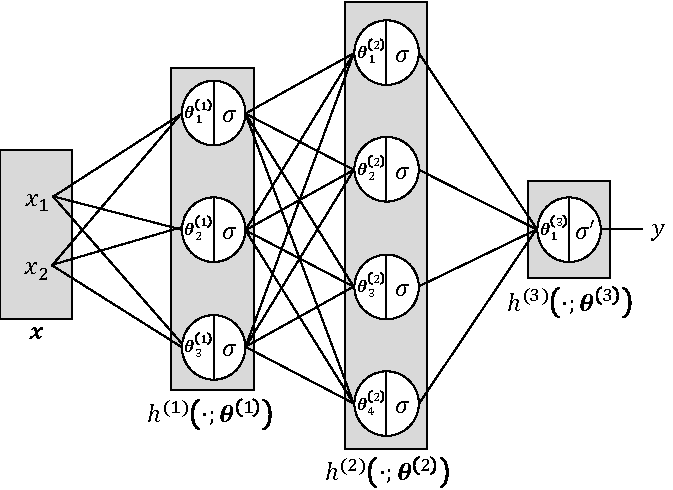
\includegraphics[width=\textwidth]{backml/mlp.pdf}
  \caption{A \acrlong{mlp} with 2 hidden layers $h^{(1)}$ and $h^{(^2)}$ for a two-dimensional input $\vect{x}$.}
  \label{fig:backml:mlp}
\end{figure}

\subsubsection{Convolutional neural networks}
\label{sssec:backml:dl:cnn}

As introduced in Section \ref{ssec:backml:shallowdeep}, \textit{\acrlong{cnn}s}
(\acrshort{cnn}) are the origin of the ``\acrlong{dl} revolution''. Despite the
recently-revived interest, \acrshort{cnn}s have been researched since the late
1980s \parencite{lecun1989handwritten}. A \acrshort{cnn} is a network containing
at least one convolutional layer. Nowadays, such layers are a core component of
all networks processing structured data (time series, images, video, etc). For
instance, in image classification, typical architectures (see Figure \ref{fig:backml:cnn})
stack several convolutional and pooling layers followed by a fully-connected
network (\ie a \acrshort{mlp}). The convolutional layer is introduced in this
section and the pooling layer in Section \ref{sssec:backml:poolinglayer}.

\begin{figure}
  \centering
  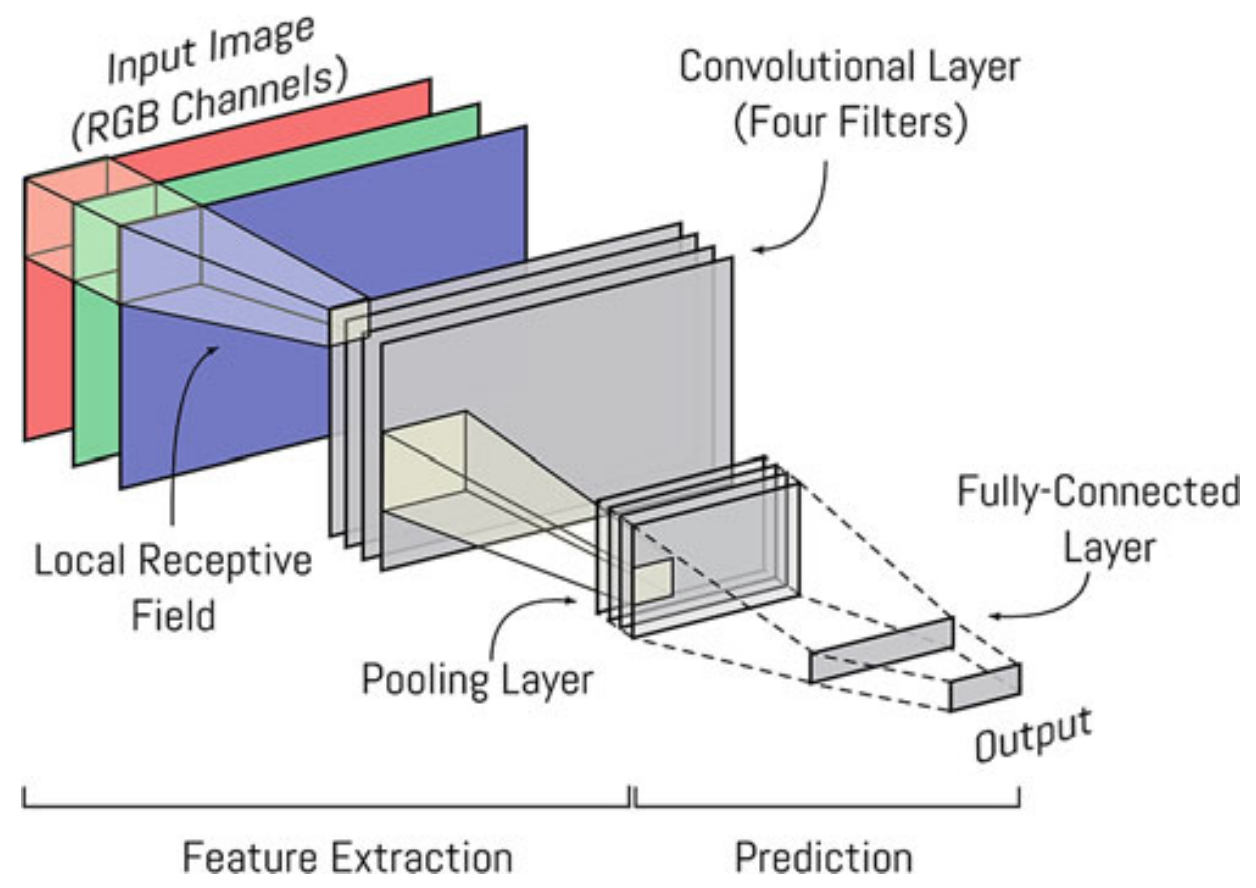
\includegraphics[width=0.75\textwidth]{backml/convnet.png}
  \caption{A \acrlong{cnn} (source \parencite{millar2019using}).}
  \label{fig:backml:cnn}
\end{figure}

Let us suppose a naive implementation of an image classifier with a \acrshort{mlp}
where each neuron in the first layer is connected to each input pixel. This model
is extremely complex and prone to overfitting, as it would realistically contain
billions of weights for a regular image. Natural images and related \acrlong{ml}
tasks have interesting properties that can be used to improve this naive model.

A first property is that \textit{pixel correlations are local}, meaning that pixels
far from each other in the image are less likely to be correlated than close
pixels. It implies that connecting individual neurons to all input pixels is
excessive and one would rather want to connect them to patches of close pixels.
A second property is that an image can be considered a \textit{stationary signal}
(\ie pixel statistics are similar at different locations of the image). Therefore,
it is relevant to use the same set of weights for all the locally-connected neurons
of a layer. These architectural choices are examples of inductive bias and motivate
the \textit{convolutional layer}. Although, we have discussed the case of images,
convolutional layers can also be generalized for 1D (\eg time series) or 3D (\eg
3D image volume) when the locality and stationarity assumptions hold.

A two-dimensional convolutional layer $h$ can be seen as a function generating an
arbitrary number $f_{out}$ of \textit{feature maps}
$\vect{a} \in \mathbb{R}^{r_{out} \times c_{out} \times f_{out}}$ from an input
$\vect{z}^{(in)} \in \mathbb{R}^{r_{in} \times c_{in} \times f_{in}}$. Feature
map $k \in \left\{1, 2, ..., f_{out}\right\}$ is the result of convoluting a
learnable weight tensor $\pmb{\theta}_k$ of dimensions $r_f \times c_f \times f_{in}$
called \textit{kernel} or \textit{filter} over the input $\vect{z}^{(in)}$:

\begin{equation}
\label{eqn:backml:convnet}
a_{ijk} = \theta_{0;k} + \sum_{s=1}^{r_f} \sum_{t=1}^{c_f} \sum_{u=1}^{f_{in}} \theta^{(l)}_{s,t,u;k} \times z^{(l-1)}_{i+s,j+t,u}
\end{equation}

where $(i, j)$ are the coordinates of a vector of $\vect{z}^{(in)}$, $\theta_{0;k}$
is the bias and $\theta^{(l)}_{s,t,u;k}$ is the weight at coordinates $(s,t,u)$
of tensor $\pmb{\theta}_k$. Similarly as for the perceptron, this linear operation
is then followed by a non-linearity:

\begin{equation}
\label{eqn:backml:convnetwithactiv}
\vect{z}^{(out)} = h\left(\vect{z}^{(in)}\right) = \sigma\left(\vect{a}\right)
\end{equation}

Convolutional layers have many hyperparameters including the number of feature
maps $f_{out}$ and filter dimensions $r_f$ and $c_f$ (typically $r_f \times c_f = 3 \times 3$
or $5 \times 5$) which both directly control the number of learnable parameters
of the layer (and therefore its complexity). In addition to those, the \textit{stride}
$s$ allows reducing the amount of computations of the layer by evaluating the
kernel every $s$ pixels (instead of every pixels) along a dimension. The
\textit{padding} defines how convolution behaves near the edges of the image where
all the considered pixels might not exist. Typical padding options are considering
missing pixels to have value 0, mirroring the image at the edge, \etc. Padding
and stride are illustrated in Figure \ref{fig:backml:paddingstride}.

\begin{figure}
  \centering
  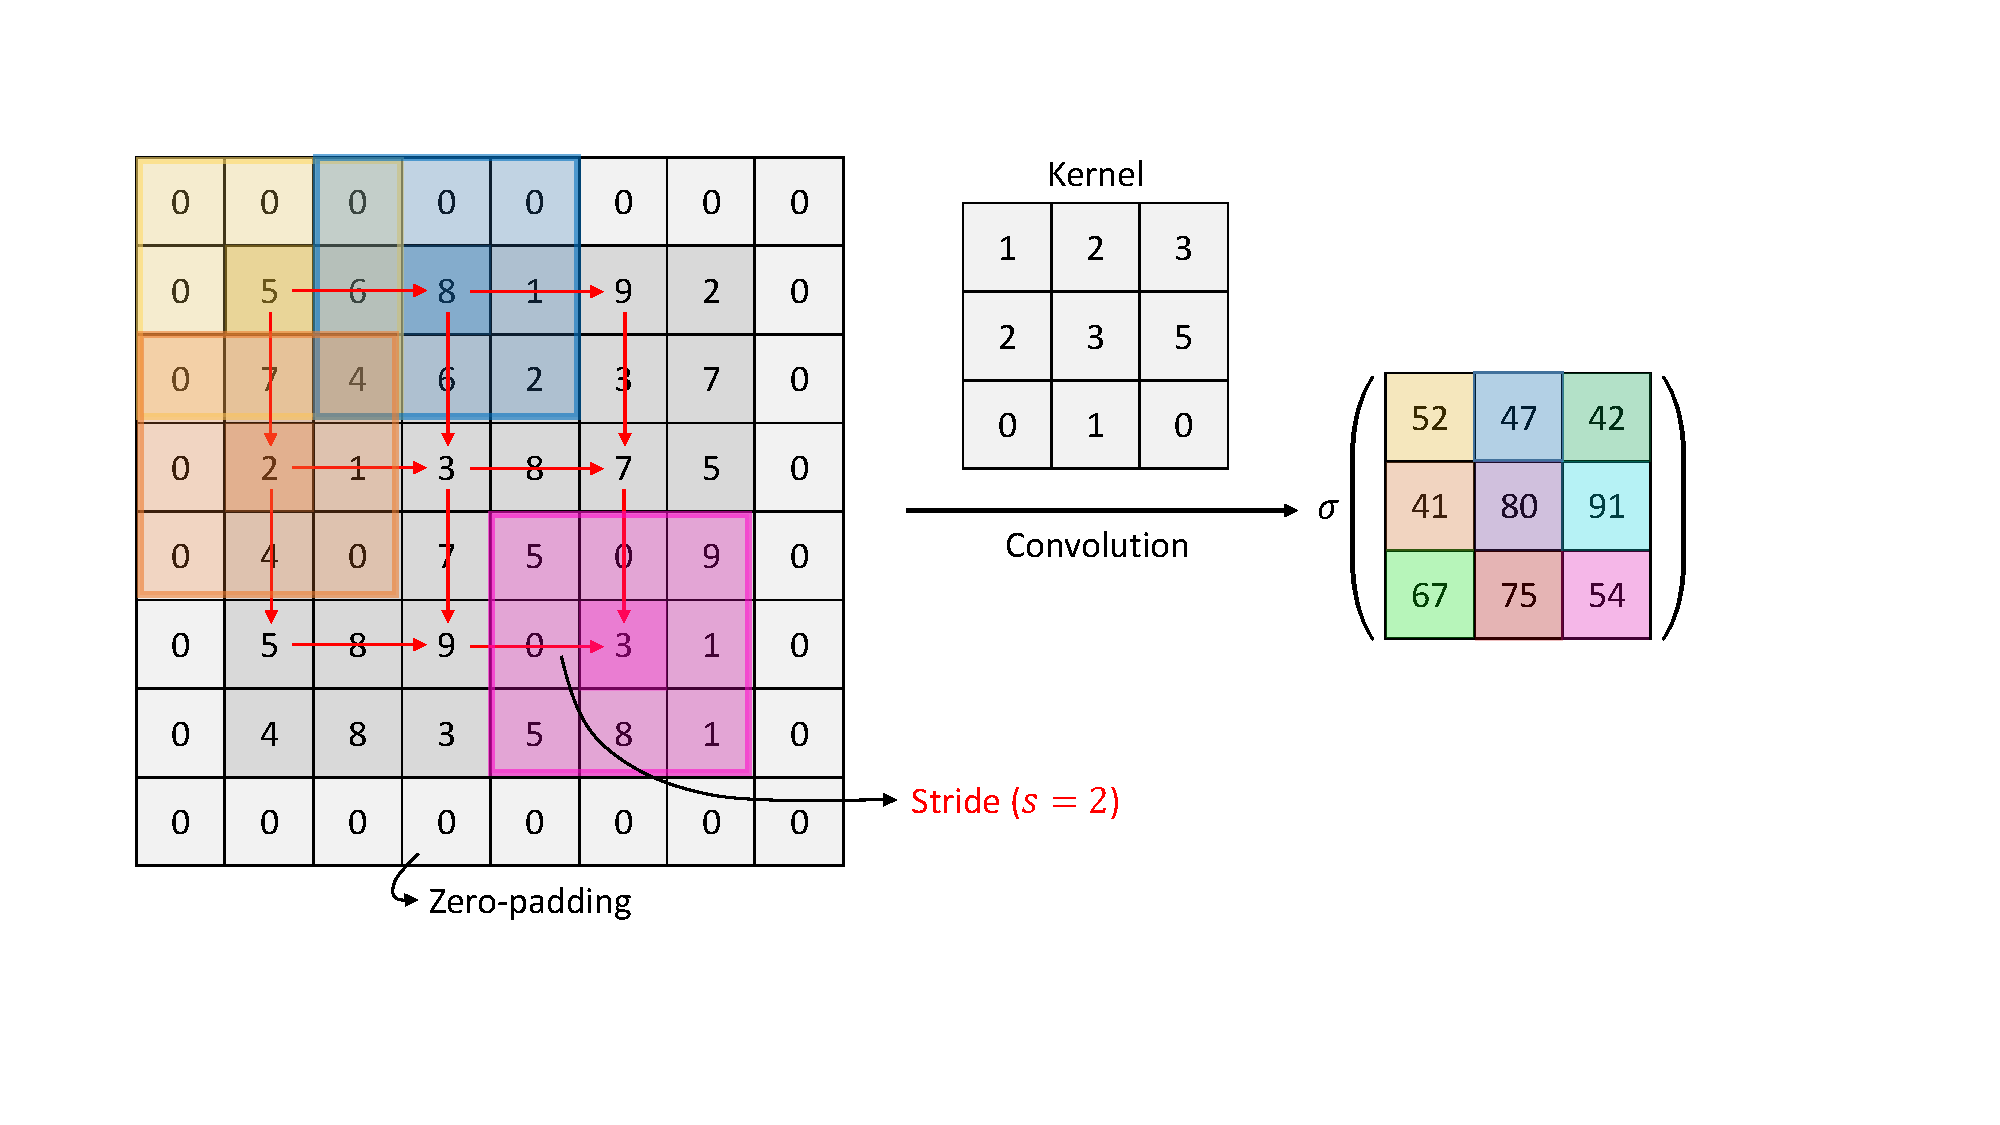
\includegraphics[width=\textwidth]{backml/convolutionwithstride.pdf}
  \caption{Illustration of stride and padding.}
  \label{fig:backml:paddingstride}
\end{figure}

In addition to exploiting locality and stationarity, \acrshort{cnn}s have other
interesting properties which contribute to their efficiency for processing structured
data. They have \textit{equivariance to translation} which means that translating
the convolutional layer input along some of the dimensions only translates the
output along the same dimensions. For tasks like image classification, object
location is often irrelevant for inferring the class. Therefore, the network does
not have to learn this invariance which makes training easier. It has also been
shown that, for image classification, the learned kernels are similar to classical
computer vision filters capturing edges or color patterns in early layers and, as
one ascends the network, kernels show compositionability, invariance and class
discrimination \parencite{zeiler2014visualizing} confirming the ability of such
a network to learn and use the inherent hierarchical structure of the data. Stacking
convolutional layers also brings the benefit of increasing the receptive field of
late layers. The receptive field of an activation $a^{(l)}_{ijk}$ in a feature
map $k$ at layer $l$ is the set of pixels of the input that influence this
activation. The larger the receptive field, the more context is considered by the
activation.

\subsubsection{Pooling layer}
\label{sssec:backml:poolinglayer}

Pooling layers are another common components of \acrshort{cnn}s. Their role is to
reduce the dimensionality of feature maps by aggregating close activations. In a
way, pooling layer can be seen as a special convolutional layer with stride of
which the kernel is not learned but rather computes a possibly non-linear statistics.
The depth of the feature maps before and after pooling does not change (\ie
$f_{in} = f_{out}$). Pooling share some hyperparameters with convolution including
stride and padding. Regarding the aggregation function, the most common choices
are \textit{max pooling} or \textit{average pooling}. The former will output the
largest activation among the one covered by the kernel:
\begin{equation}
\label{eqn:backml:maxpooling}
a_{ijk} = \text{max} \left\{ x_{i+s,j+t,k} \mid s = 1, ..., r_f; t = 1, ..., c_f \right\}
\end{equation}
The latter will average the activations covered by the kernel:
\begin{equation}
\label{eqn:backml:avgpooling}
a_{ijk} = \frac{1}{r_f \times c_f} \sum_{s=1}^{r_f} \sum_{t=1}^{c_f}  x_{i+s,j+t,k}
\end{equation}

Pooling, similarly to convolution, brings equivariance to translation and increase
the receptive field of deeper layers. The reduction of dimensionality also reduces
the computational cost of the network as deeper layers have smaller feature maps
to process. There exist other types of pooling layers which are described in
\parencite{gholamalinezhad2020pooling}.

\subsection{Neural network optimization}
\label{ssec:backml:dl:opti}
Remains the question of how to find the best parameters for the neural network
$h(\cdot; \theta)$ using a training set. Obviously, these weights should be tuned
so that the final model minimizes the expected risk (\ie the generalization error)
which is not directly possible as explained in Section \ref{ssec:backml:modelselection}.
Following the \acrshort{erm} principle, $h(\cdot; \theta)$ can be optimized by
minimizing its error on the training set measured by a loss $\mathcal{L}$. In most
cases, it is not possible to find the solution analytically and, therefore, one
resorts to numerical optimization and variants of \textit{gradient descent}
algorithms.

Starting from initial model parameters $\theta_0$, gradient descent is an algorithm
that iteratively builds a sequence of parameters $\theta_i$ such that the loss
should ideally decrease when $i$ increases. Every iteration, the parameters are
updated by applying them a correction in opposite direction of the gradients of
$\mathcal{L}$ in the parameters space:
\begin{equation}
\label{eqn:backml:gradientdescent}
\theta_{i} = \theta_{i-1} - \gamma \nabla \mathcal{L}(h(\cdot, \theta_{i}))
\end{equation}
where $\gamma$ is the learning rate, an hyperparameter for tuning the amplitude
of the parameters update.

Gradient descent does not guarantee convergence to a global minimum in general as
the optimization can either reach a local minimum or diverge. The choices of
$\theta_0$ and $\gamma$ are important to avoid divergence. Regarding the local
minima issue, the very high-dimensional nature of neural networks makes it unlikely
to have no dimension along which the model can improve at a given iteration.
Moreover, finding parameters that achieve the global minimum of the training loss
is generally unwanted as it might lead to overfitting.

At every iteration, the original gradient descent algorithm computes gradients
over the whole training set which is particularily inefficient when $n \gg$. A
way of improving this consists in using \acrfirstit{sgd} where the gradients are
approximated using a subset $\mathcal{B}$ of training samples called a \textit{batch}
instead of the whole set. This approach has been shown to be particularily efficient
for both generalization of the model and computational cost of training
\parencite{bottou201113}. When $1 < |\mathcal{B}| < n$, \acrshort{sgd} becomes
\textit{mini-batch gradient descent} which is the most used optimization strategy
for training neural networks nowadays. The batch size is often chosen based on
practical considerations like the amount of memory available on the hardware
running the learning algorithm.

Several adjustements to the gradient descent formulation of Equation
\ref{eqn:backml:gradientdescent} have shown to be effective for convergence and
stability of the optimization. In the thesis, whenever we optimize a neural network
by gradient descent, we use the Adam optimizer \parencite{kingma2014adam} approach
which normalizes the gradients using moving estimates of their mean and uncentered
variance. This method is efficient and does not require much tuning of the
hyperparameters yet makes training more robust.

\subsubsection{Backward propagation}
\label{sssec:backml:backprop}

Gradient descent, as its name suggests, heavily relies on gradient of parameters
for updating the model. The success of deep learning can be partly attributed to
an efficient algorithm for computing these gradients called \textit{backward propagation}
\parencite{rumelhart1986learning} (\aka backpropagation). The algorithm is based
on the \textit{chain rule} which states that the derivative of a composition of
functions $y(x) = (h^{(L)} \circ h^{(L-1)} \circ ... \circ h^{(1)})(x)$ with respect
to its input can be broken down into a product of derivatives. Given
$y_i = (h^{(i)} \circ h^{(i-1)} \circ ... \circ h^{(1)})(x)$, the composition of
the $i^{\text{th}}$ first functions ($i = 1, ..., L$), the chain rule states
that:

\begin{equation}
\label{eqn:backml:chainrule}
\nabla h = \dfrac{\partial h(x)}{\partial x} = \dfrac{\partial y_L}{\partial x} = \dfrac{\partial y_L}{\partial y_{L-1}} \times ... \times \dfrac{\partial y_2}{\partial y_1} \times \dfrac{\partial y_1}{\partial x}
\end{equation}

This applies directly to feedforward neural networks which are compositions of
functions and implies that computing the parameters gradients can be broken down
into computing local gradients at every layer. The backward propagation algorithm
starts from the loss and iteratively evaluates local gradients going backward in
the network until all parameters have been reached. These local gradients can then
be combined using the chain rule and the resulting gradients can be used to update
the parameters as dictated by gradient descent. This obviously requires that all
functions $h^{(l)}$ are differentiable as introduced in Section
\ref{ssec:backml:dp:components}.

Relying on gradients of a long chain of functions for the optimization can be
troublesome at times. Indeed, when a neural network is not build carefully,
\textit{vanishing} or \textit{exploding gradients} can appear. Some activation
functions such as the hyperbolic tangent or the sigmoid have saturating modes as
they converge to constant values. As these fonctions converge towards a constant,
their derivatives become smaller and smaller and converge to zero. Because of the
multiplicative nature of the chain rule, one gradient in the chain is enough to
cancel all gradients upstream which happens when the activations start working in
their saturating regime. There exist best practices to reduce the likelihood of
vanishing gradients: weights must be carefully initialized, it is better to avoid
activation functions with saturating modes (\acrshort{relu} is a good candidate)
and some architectural tricks can help (see Sections \ref{sssec:backml:batchnorm}
and \ref{sssec:backml:arch:residual}). In opposition, exploding gradients cause
divergence because gradients are too large. Again architectural tricks, careful
weigths and learning rate initilization makes this issue less likely to occur.

Nowadays, all deep learning frameworks implement backward propagation and also
feature automatic differentiation. Automatic differentiation means that every
basic mathematical function present in the library is associated with its analytical
derivative. Therefore, during backpropagation, the algorithm can compute the
gradients automatically and exactly based on this information. The combination of
these two features makes training a neural network particularily easy as everything
is automated.

\subsubsection{Batch normalization}
\label{sssec:backml:batchnorm}

The \acrfirstit{bn} \parencite{ioffe2015batch} layer is part of the family of
normalization layers. This layer acts as a regularizer and is usually placed before
activations in neural networks. Given a signal
$\vect{x} = \left(\vect{x}_1, \vect{x}_2, ..., \vect{x}_f\right) \in \mathbb{R}^f$
(\eg the output of a convolutional layer), the \acrshort{bn} layer maintains an
estimate of the mean $\mu_i$ and variance $\sigma_i$ ($i = 1, ..., f$) of the
preceeding layer output computed over the batch. These estimates are used to
normalize the inputs into an intermediate signal $\hat{\vect{x}}$. Obviously,
whether this normalization is actually beneficial for the network is task-, layer-
and feature-dependent and there are probably scenarii where normalizing would hurt
performance. Therefore, the signal $\hat{\vect{x}}$ is then followed by a learnable
linear layer allowing the network to learn to revert this normalization if
necessary:
\begin{equation}
\label{eqn:backml:bn}
\acrshort{bn}(\vect{x}) = \begin{bmatrix}
\alpha_1 \left(\dfrac{\vect{x}_1 - \mu_1}{\sqrt{\sigma^2_1 + \epsilon}}\right) + \beta_1 & ... & \alpha_f \left(\dfrac{\vect{x}_f - \mu_f}{\sqrt{\sigma^2_f + \epsilon}}\right) + \beta_f \\
\end{bmatrix}\end{equation}
where the $\alpha_i$ and $\beta_i$ are learnable parameters. During training,
the input statistics $\mu_i$ and $\sigma_i$ are computed on-the-fly using moving
averages. At inference, the statistics are frozen as well as the learnable parameters
$\alpha_i$ and $\beta_i$.

Batch normalization greatly helps network optimization by maintaining intermediate
activations within acceptable ranges of values and therefore reducing the risk of
vanishing or exploding gradients, narrowing the parameter search and allowing
higher learning rates.

Unfortunately, the use of batch statistics can also be an issue. When there is a
sudden change in the model input distribution, the batch statistics are likely to
change quickly but the linear layer, restricted by the learning rate, will probably
not be able to adapt as quickly. This can cause instabilities while the networks
adapts its \acrlong{bn} layers for the new distribution. This situation can occur
for instance with \acrlong{tl} where source and target tasks can have drastically
different input distributions.

\TODO{explain our solution here for batchnorm in transfer issue? or section on in deep \acrlong{tl} ? or in multi task chapter?}

\subsection{Modern network architectures}
\label{ssec:backml:dl:modernarchi}

This section presents different architectures used in our contributions.

\paragraph{Simple layer-stacking architecture}
\label{sssec:backml:arch:layerstacking}
After the success of AlexNet, researchers investigated the effect of model depth
on classification performance. An architecture in particular caught the attention
by ending up a runner up for a later edition of \acrshort{ilsvrc} in 2014. This
architecture is named VGG \parencite{simonyan2014very} after the team who participated
the challenge. It has two implementations we use in this thesis: VGG16 and VGG19.
The number is the count of layers with trainable weights in the architecture.
These architectures are pretty straightfoward (see Figure \ref{fig:backml:vgg})
as they only stack blocks of few convolutional layers with \acrshort{relu} activation
followed by pooling. The last convolutional layer is followed by a 3-layers
\acrshort{mlp}.

\begin{figure}
  \centering
  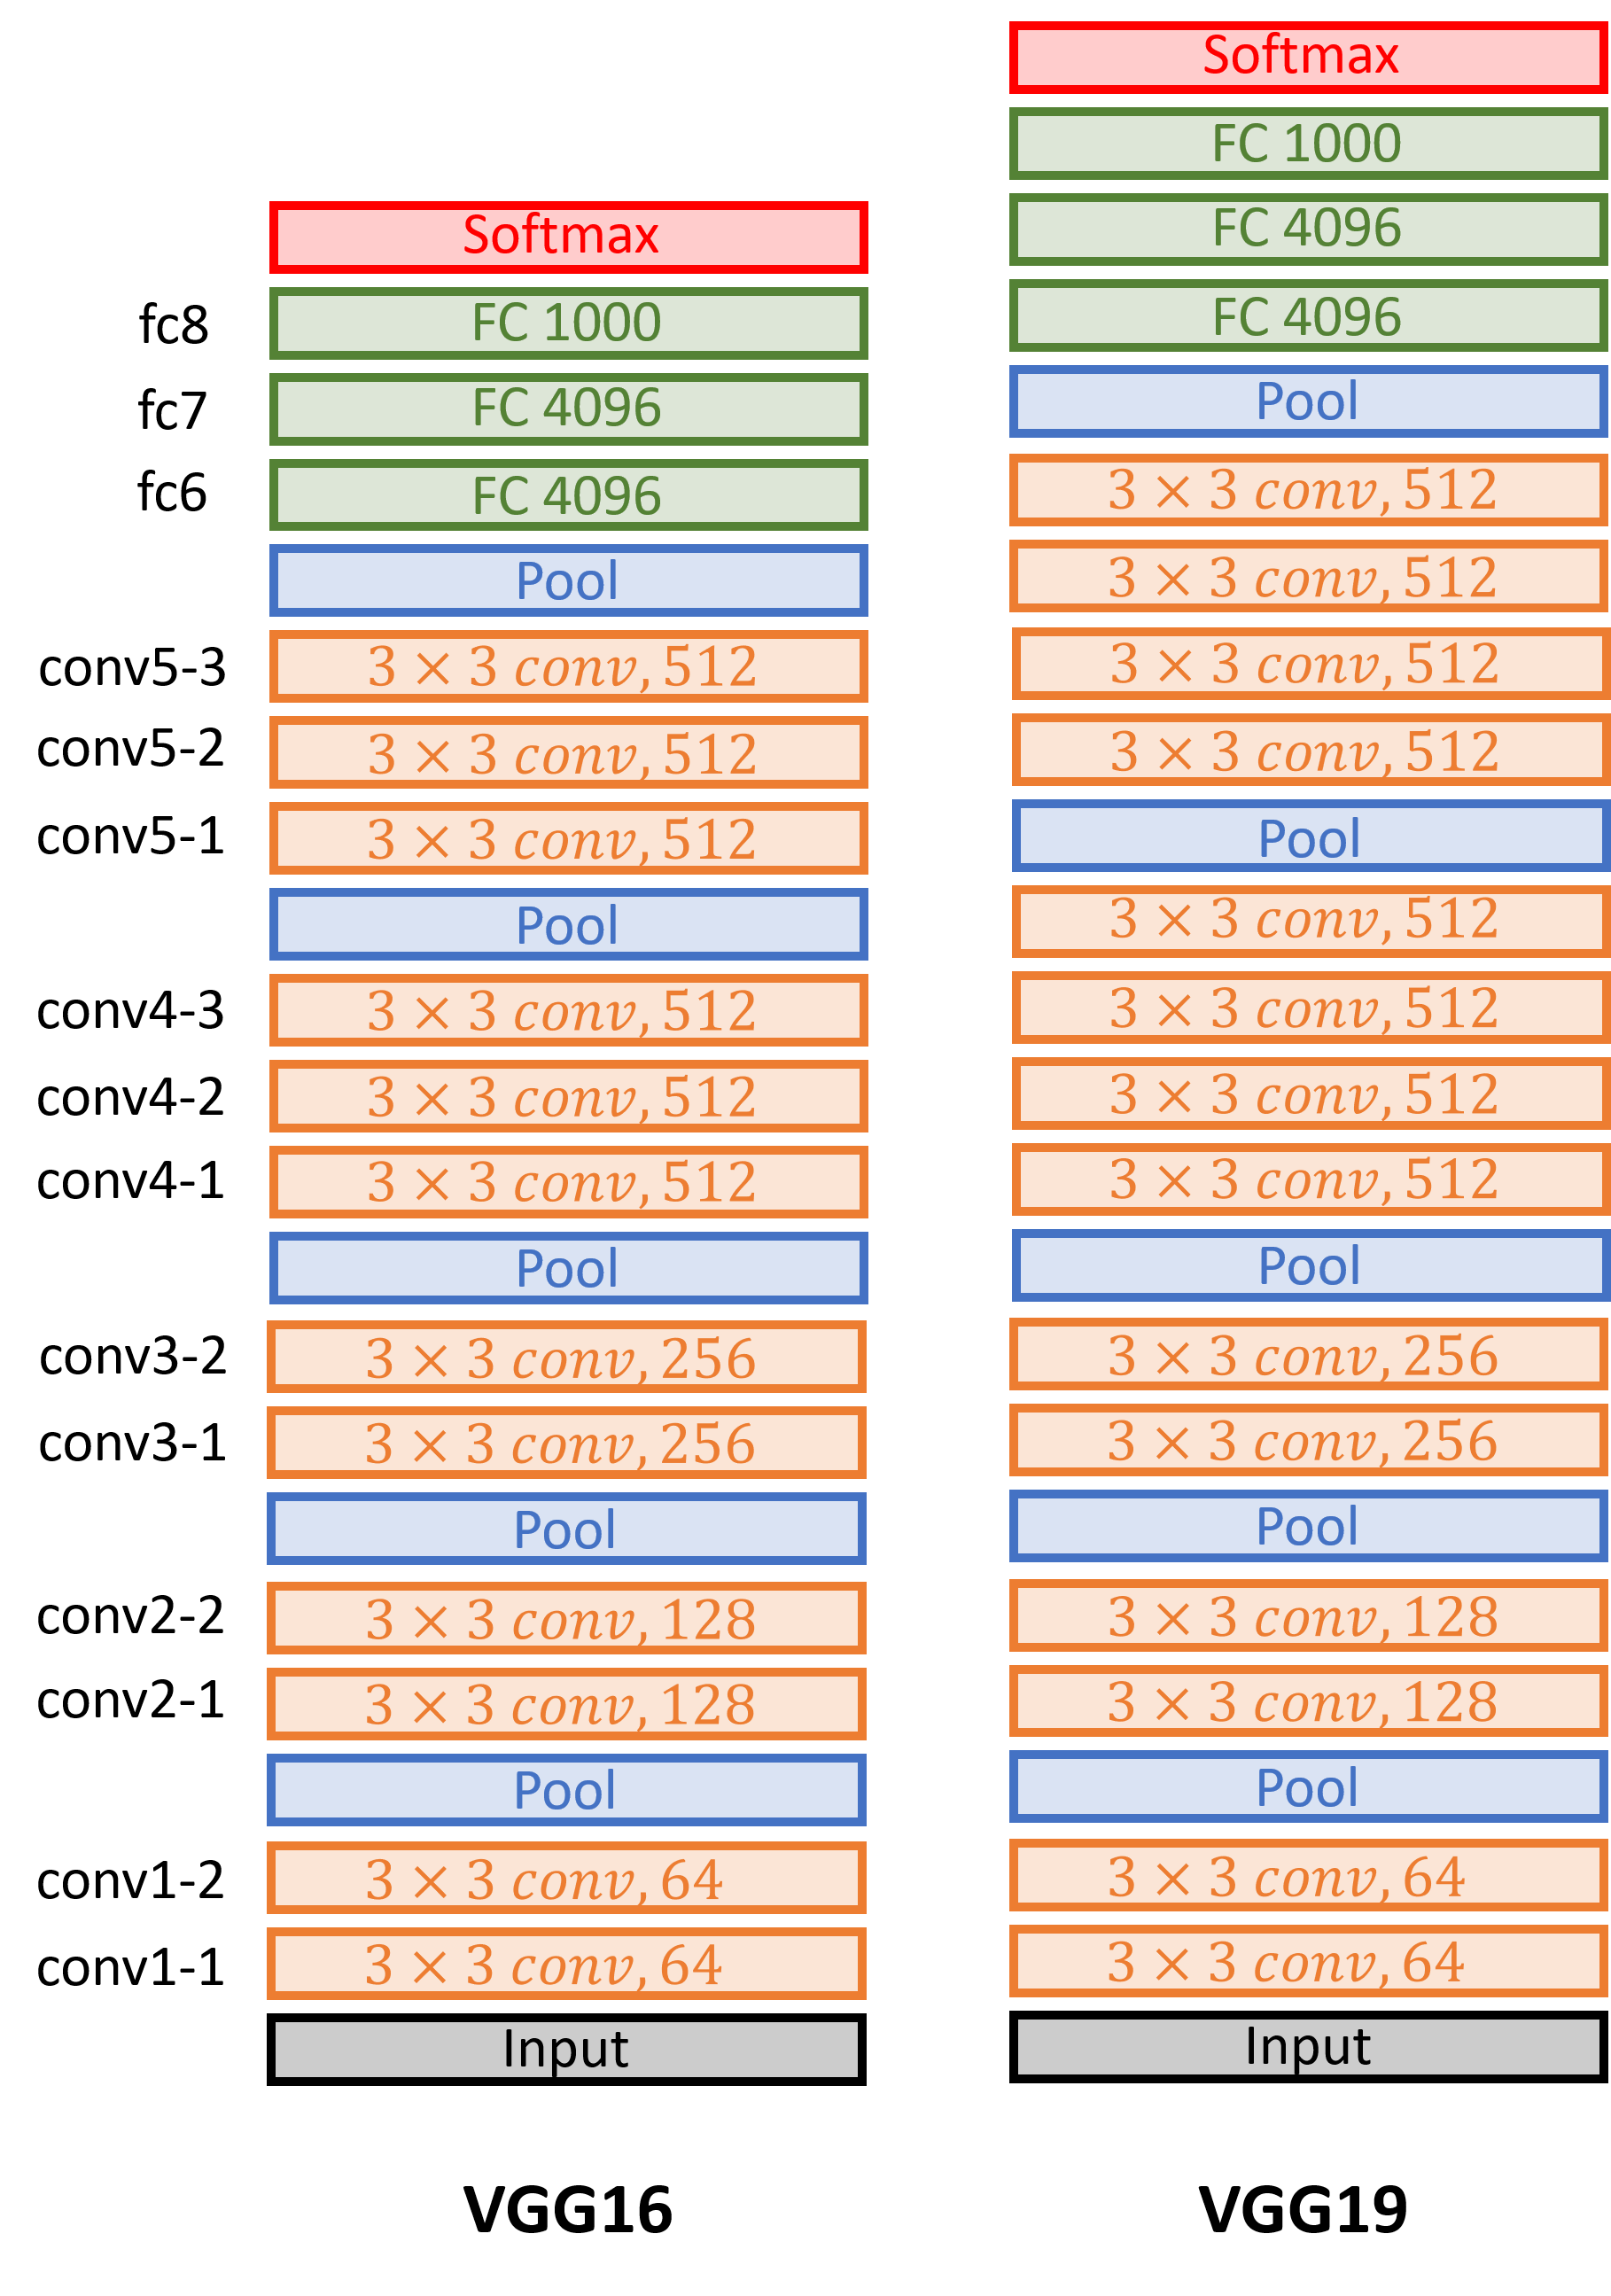
\includegraphics[rotate=-90, scale=0.28]{backml/vgg1619.png}
  \caption{VGG16 and VGG19 architectures (source: \parencite{img:vgg1619})}
  \label{fig:backml:vgg}
\end{figure}

\paragraph{Residual architecture}
\label{sssec:backml:arch:residual}

Although improving over AlexNet, very deep networks like VGGs are subject to
training difficulties: beyond a certain model depth, accuracies sometimes start
to decrease. This can be attributed to the fact that, for a given task, adding
layers beyond a certain depth is not necessary. Moreover, it can be difficult for
gradients to flow back given the depth of the architecture (\ie vanishing gradients).
In order to address those two issues, ResNet \parencite{he2016deep} introduces
the \textit{residual mapping}, or \textit{skip-connection}. Given a layer
$h^{(l)}(\vect{x})$, the residual mapping $r^{(l)}(\vect{x})$ would be:
\begin{equation}
\label{eqn:backml:residual}
r^{(l)}(\vect{x}) = \vect{x} + h^{(l)}(\vect{x}).
\end{equation}
This residual mapping makes it easier for the optimizer to simply ignore the layer
as it just has to tune all the weights in $h^{(l)}(\vect{x})$ to 0 in which case
$r^{(l)}(\vect{x}) = \vect{x}$. Moreover, gradients are still able to flow freely
through the skip connection. This increased trainability has been empirically
confirmed as very deep residual network (up to 150 layers) have won \acrshort{ilsvrc}
in 2015 and 2016 and have shown impressive performance in many other contexts.
Another advantage of residual networks is that, even though they are deeper than
their VGG counterparts, they need much less parameters to reach better
performance\footnote{VGG16 and 19 have more than 140M parameters whereas ResNet50 has 25M and the largest ResNet152 has 66M parameters.}
making ResNets more lightweight. Nowadays, residual connections are a common
building block in deep architectures. In this thesis, we use one of the first
iteration of ResNets, namely ResNet50 (see Figure \ref{fig:backml:resnet} for
ResNet34, a similar architecture).

\begin{figure}
  \centering
  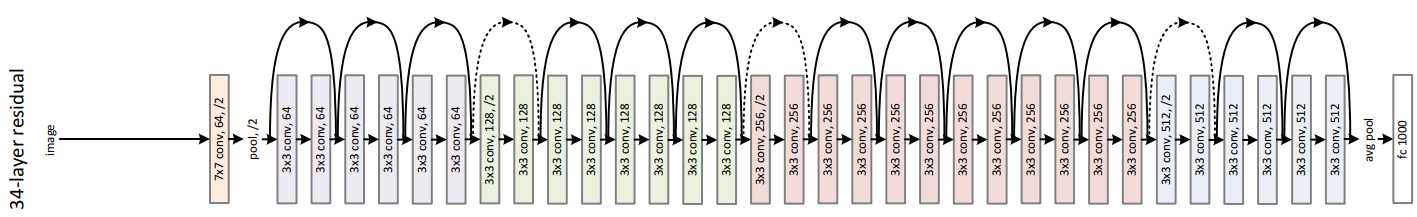
\includegraphics[width=\textwidth]{backml/resnet34.png}
  \caption{ResNet34, same design as ResNet50 but less layers. Residual connections are placed every two convolutional layers (source: \parencite{he2016deep}).}
  \label{fig:backml:resnet}
\end{figure}

\paragraph{Inception architecture}
\label{sssec:backml:arch:inception}
% InceptionV3
% InceptionResNetV2
The winning method of \acrshort{ilsvrc}2014 was based on an architecture called
GoogLeNet \parencite{szegedy2015going} (\aka InceptionV1). This architecture is
based on \textit{inception modules}. An inception module is a composition of
convolutional layers built to maintain a certain level of representativeness while
reducing the number of training parameters compared to a block of plain convolutional
layers. An example of a trick used to reduce the number of parameters is to use
two consecutive $3 \times 3$ instead of one $5 \times 5$ convolutional layers. In
this thesis, we use InceptionV3 \parencite{szegedy2016rethinking}, the third
iteration of the architecture, which essentially scales it up by using factorized
convolutions and regularization. We also use InceptionResNetV2, a version of the
Inception architecture using residual connections
\parencite{szegedy2017inception}.


\paragraph{Dense architecture}
\label{sssec:backml:arch:dense}
The densely connected convolutional networks \parencite{huang2017densely} push
further the idea of residual connection. Let us suppose a group $g$ of $L$
consecutive convolutional layers $h^{(l)}$ ($l = 1, ..., L$) taking $\vect{x}$ as
input. In this group, each layer $h^{(l)}$ receives as input the outputs of all
preceeding layers $h^{(i)}$ ($i = 1, ..., l-1$) and the input signal $\vect{x}$.
This group $g$ is called a \textit{dense block} and is the basis for the densely
connected networks. Such networks typically stack several dense blocks connected
together with one convolution and one pooling layers (see Figure
\ref{fig:backml:densenet}).

\begin{figure}
  \centering
  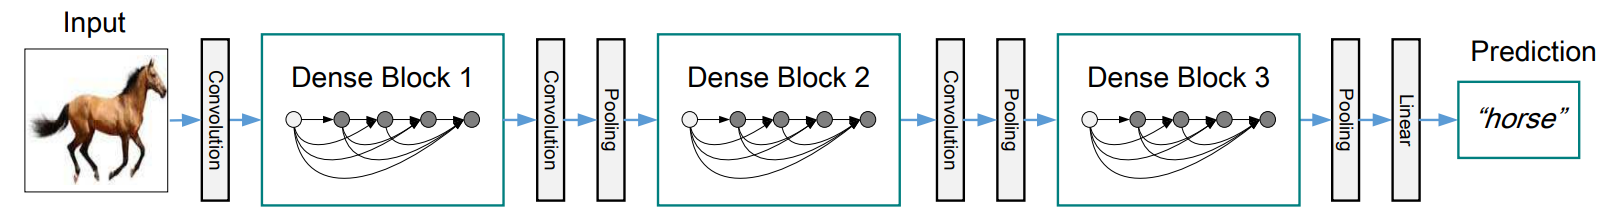
\includegraphics[width=\textwidth]{backml/densenet.png}
  \caption{A densely connected network (source: \parencite{huang2017densely}).}
  \label{fig:backml:densenet}
\end{figure}

\paragraph{A segmentation architecture, UNet}
\label{sssec:backml:arch:segment}

For tackling image segmentation tasks, one generally uses \textit{\acrlong{fcn}s}
(\acrshort{fcn}) which is a kind of network where (almost) all layers are
convolutional. One of the most popular architecture for segmentation is a U-shaped
network called U-Net \parencite{ronneberger2015unet}. This architecture is composed
of a contracting and an expanding paths (hence the ``U'', see Figure
\ref{fig:backml:unet}). Similarly as for classification networks, the former is
composed of convolutional and pooling layers that progressively encodes the input
images into high-level context features. The latter combines decoded high-level
features with low-level features from the expanding path to eventually generate
a segmentation map. The decoding of low-level features is learned using an
upconvolution layer. Upconvolution is a layer that upsamples a signal with a
learnable filter. In order to combine decoded high level features and low-level
features, U-Net uses skip connections from the contracting to the expanding
paths.

\begin{figure}
  \centering
  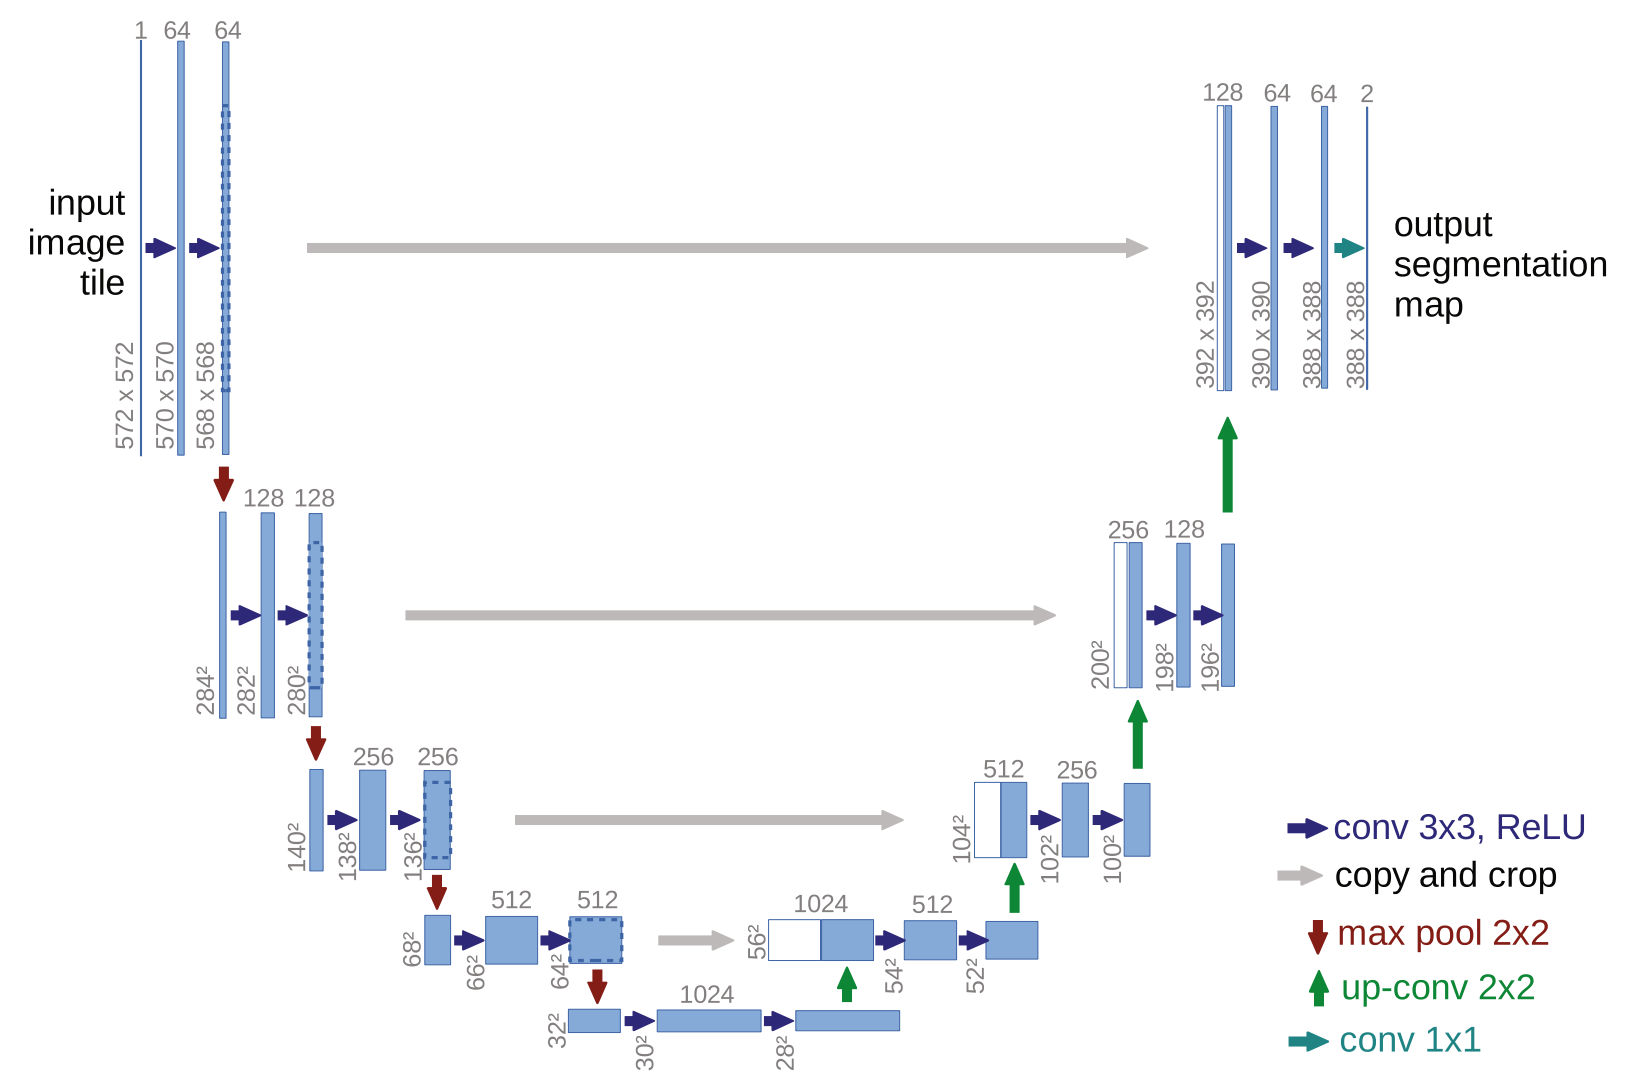
\includegraphics[width=\textwidth]{backml/unet.png}
  \caption{U-Net architecture (source: \parencite{ronneberger2015unet}).}
  \label{fig:backml:unet}
\end{figure}

\subsection{Deep transfer learning}
\label{ssec:backml:dl:deeptransfer}

As presented in Section \ref{ssec:backml:transfer}, \acrlong{tl} regroups several
families of methods which have been and continue to be explored through the prism
of \acrlong{dl} \parencite{tan2018survey}. In this thesis, we focus on supervised
model-based (or network-based) \acrlong{tl} applied to image classification. With
this approach, knowledge is encoded through the parameters of a model. This model
is first trained on a source task, usually a large image classification dataset,
then transfered to the target task.

There are two approaches for transfering a deep neural network to a target task.
Let us consider three networks $h_s$, $h_o$ and $h_n$ respectively parametrized
by $\theta_s$, $\theta_o$ and $\theta_n$. In the remaininder of this section, we
will designate a network interchangeably by its set of parameters $\theta_i$ or
its function $h_i(\cdot;\theta_i)$. The network $\theta_s$ is shared between the
source and target tasks and $\theta_o$ and $\theta_n$ are the task-specific
networks. Both approaches first require the network $h = h_o \circ h_s$ to be
trained on the source task. At the end of training, $\theta_s$ encodes the knowledge
to be transfered.

\begin{figure}
  \centering
  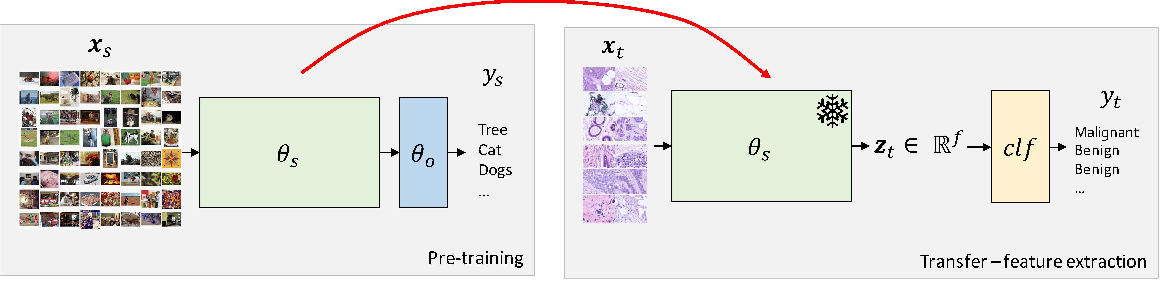
\includegraphics[width=\textwidth]{backml/transfer-fe.pdf}
  \caption{Supervised \acrlong{tl} by \textit{feature extraction}. The shared network is trained by supervised learning on the source task. Then, the shared part $\theta_s$ is extracted and used as an encoder for images of the target task. A third-party classifier $clf$ can be trained and used to classify the encoded target data.}
  \label{fig:backml:transfer-fe}
\end{figure}

The first transfer approach is \textit{feature extraction} (see Figure
\ref{fig:backml:transfer-fe}) and simply consists in generating a new representation
for samples of the target task using $\theta_s$ as an encoder. For each sample
$\mathbf{x}_i$ of the target task, this encoder generates a feature vector
$\vect{z}_i = h_s(\vect{x}_i;\theta_s) \in \mathbb{R}^f$ where $f$ is the number
of features. The encoder is said to be ``\textit{frozen}'' as it is not updated
after transfer. The generated features can be used to train a third-party classifier
on the target task which can be as simple as a linear model. A common choice of
classifier is a linear \acrshort{svm}.

\begin{figure}
  \centering
  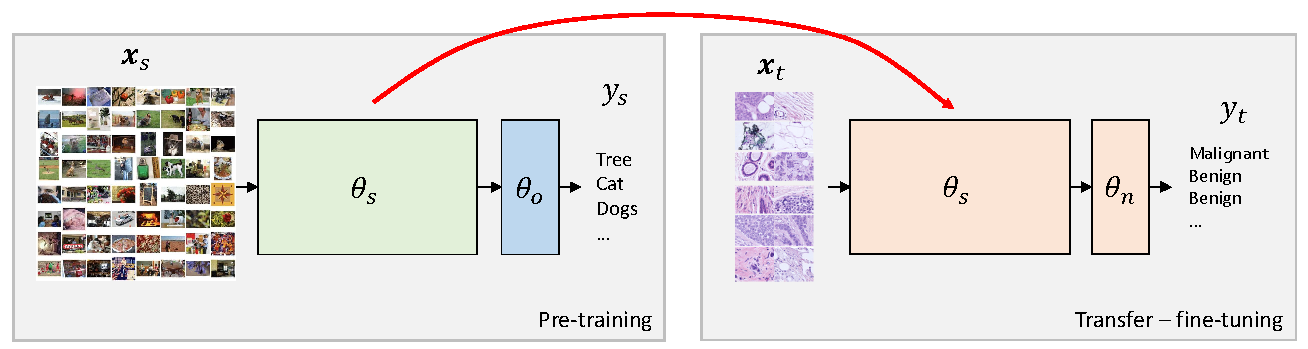
\includegraphics[width=\textwidth]{backml/transfer-ft.pdf}
  \caption{Supervised \acrlong{tl} by \textit{fine-tuning}. The shared network is trained by supervised learning on the source task. Then, the shared part $\theta_s$ is extracted and attached to $\theta_n$. The network $h_n \circ h_s$ is trained by gradient descent on the target task.}
  \label{fig:backml:transfer-ft}
\end{figure}

The second transfer approach is \textit{fine-tuning} (see Figure \ref{fig:backml:transfer-ft})
where the task-specific part of the network $\theta_{o}$ is replaced by a new
classification network $\theta_{n}$ and the resulting network $h = h_c \circ h_s$
is further trained by gradient descent on the target task. Subjecting the whole
network to gradient descent will change the features learned on the source task
which can cause catastrophic interference. Therefore, a way of alleviating the
issue is to use a small learning rate (compared to the initial training learning
rate). Another of way preventing this issue consists in freezing a part of
$\theta_s$, usually the first layers.

The feature extraction approach only emerged recently with works on the Overfeat
\parencite{sermanet2013overfeat, razavian2014cnn} and Decaf \parencite{donahue2014decaf}
convolutional architectures. The authors trained their AlexNet-based networks in
a supervised manner on the large ImageNet source dataset composed of 1.2 millions
natural images and 1000 distinct classes. They both showed that these networks
were able to produce discriminative features for tasks they were not trained on.

Building upon these results, \parencite{yosinski2014transferable} analyzed the
transferability of deep neural networks using both approaches in more details.
Their most prominent conclusion is that features in a neural network become less
transferable as one moves deeper in the network indicating that the network features
shift from generic to specific along the network. This result is consistent with
\parencite{zeiler2014visualizing} as early layers typically learn classical computer
vision filters. This motivates freezing only the first layers of the network to
avoid catastrophic interference as they are more generic and therefore should not
require much tuning. They also studied how task similarity impacted transfer
performance and found that similar tasks indeed benefited better from transfer
than dissimilar ones. This was confirmed in \parencite{mensink2021factors} who 
showed that for a variety of tasks, there exists a source task that outperforms
ImageNet, especially when this task incorporates in some ways the target domain.
More recently, \parencite{kornblith2019better} showed that there is a correlation 
between model performance on the source task (in this case  ImageNet) and transfer 
performance on the target task. 

Whereas the versatility of ImageNet initially fueled research in deep \acrlong{tl}
with supervised model pre-training, several recent contributions have shown that
pre-training could be performed differently. For instance, SimCLR \parencite{chen2020simple}
uses contrastive learning to learn the model. This is a self-supervised approach
which consists in generating pairs of similar and dissimilar images using data
augmentation and training a network to discriminate these pairs. They have shown
that the resulting network has learned discriminative features that can be transfered
quite efficiently to new tasks. The \acrfirstit{vit} \parencite{dosovitskiy2020image}
is another approach based on transformers, a recent and popular family of
attention-based methods. Attention is a mechanism of selection of information
which can be implemented in different ways in neural networks \parencite{niu2021review}.
It has initially been applied with great successes on \acrfirstit{nlp} problems
but \acrshort{vit} has shown that attention-based architectures are also applicable
to vision. In this framework, the transfer process is very similar to supervised
pre-training as the model is first trained in a supervised manner on a large
database, then transfered to the target task. The only difference is that the
attention-based network does not use convolution and takes as input a sequence of
non-overlapping patches of the image. Other contributions focus on improving
classical supervised pre-training approach. For instance, \parencite{wang2019pay}
combine \acrlong{tl} and model compression as the fine-tuning process excludes
non-informative feature maps from the final model based on their \acrfirstit{afds}
mechanism.

Because of its ability to tackle data scarcity, \acrlong{tl} has been a method of
choice in many applications where this problem occurs. In Section \ref{ssec:backdp:tl},
we explore further applications of \acrlong{tl} to \acrlong{dp} and medical imaging
in general.

\subsection{Multi-task learning}
\label{ssec:backml:dl:deepmultitask}

\TODO{write}

\subsection{Self-training}
\label{ssec:backml:dl:selftraining}

As introduced in Section \ref{ssec:backml:inbetween}, self-training is a family of \acrlong{ssl} methods. A self-training process is iterative where a typical iteration consists in using a teacher model to produce pseudo-labels for unlabeled samples from $\mathcal{D}_u$ which are then combined with labeled samples from $\mathcal{D}_l$ to train a student model. 

There are several elements that characterize a self-training algorithm. An important element is the way the student and teachers models interact during the process. A common approach consists in using the current student as a teacher for the next training round, during which a new student is trained from scratch \parencite{yarowsky1995unsupervised, xie2020self}. A different approach consists in building a teacher of which the model parameters are a moving average of the student parameters at the end of each training round \parencite{tarvainen2017mean}. \cite{pham2021meta} update both the student and teacher networks by back-propagation during the self-training round. 

Another characteristic element is how the algorithm exploits the pseudo-labels. Some techniques use pseudo-labels \textit{uncertainty} to select which samples should be included for the next training rounds by excluding high entropy samples for instance \parencite{grandvalet2004semi, lee2013pseudo}. Another way of exploiting the pseudo-labels in the training signal is to exploit \textit{consistency}. Several self-training approaches ensure consistency between the predictions of the teacher and of a noisy student \parencite{xie2020self, zhu2020improving, sohn2020fixmatch, tarvainen2017mean}. The student is said to be noisy because of the stochastic nature of the data augmentation and network training (\eg caused by dropout, stochastic depth). \parencite{laine2016temporal} propose a variation of this by enforcing consistency between the current model and the pseudo-labels generated and aggregated over the past training rounds (so-called temporal ensemble).

\section{Wrapping up}
\label{sec:backml:wrapup}

In the previous sections, we gave an overview of different topics. We can now position our work in this context. In Chapters \ref{chap:comp}
and \ref{chap:mtask}, both contributions explore heterogeneous model-based
\acrlong{tl} by transfering \acrlong{dl} classification models. We use several
target tasks to study how \acrlong{tl} performs in the context of \acrlong{dp}
(more on this in Chapter \ref{chap:backdp}). The first contribution studies transfer
from ImageNet. Motivated by the fact that transfer works better when the source
and target tasks are related, the second contribution use homogeneous features-based
\acrlong{mtl} as a way to pre-train a model for transfer on \acrlong{dp} data
directly.

In Chapter \ref{chap:strain}, we move to a different type of task: image segmentation.
Working with an sparsely-annotated \acrlong{dp} dataset, we use self-training to
complete the areas where annotations are missing. We train a U-Net segmentation
model on the self-annotated segmentation.

\TODO{chapter on software contributions}
